\documentclass[12pt]{article}
\usepackage{geometry}
\geometry{a4paper, margin=2.5cm} 
%\usepackage[parfill]{parskip} 
\usepackage{amssymb}
\usepackage{amsmath}
\numberwithin{equation}{subsection}
\usepackage{amsthm}
\usepackage{setspace}
\usepackage{caption}
\usepackage{cancel}
%\setstretch{1.2}
\usepackage{graphicx}
\DeclareGraphicsExtensions{.pdf,.png,.jpg}
\usepackage{relsize}
%\usepackage{times}
\usepackage{hyperref}
\usepackage{letltxmacro}
\usepackage[reflist=true,style=windycity]{biblatex}
\addbibresource{refs.bib}
\urlstyle{same}

\newtheorem{theorem}{Theorem}
\newtheorem{proposition}{Proposition}

\theoremstyle{definition}
\newtheorem{definition}{Definition}
\newtheorem{algorithm}{Algorithm}


\DeclareMathOperator*{\argmax}{arg\,max}
\DeclareMathOperator*{\argmin}{arg\,min}



\begin{document}
\title{Memphis}
\date{\today}
\author{Max Kapur\footnote{\emph{Email:} \href{mailto:maxkapur@snu.ac.kr}{maxkapur@snu.ac.kr}}}



\maketitle

\begin{abstract}
Abstract
\end{abstract}

\pagebreak
\tableofcontents

\pagebreak
\section{Introduction}
This article considers a kind of admissions market that has not received much attention in the school-choice literature but approximates the admissions procedure used in many systems around the world. In this market, all schools have the same preference order, and students' preference orders are determined by the multinomial logit (MNL) choice model.

The primary reason for choosing this market is that it admits an expression for the demand that is invertible in the other parameters, allowing us to compute the cutoffs at Walrasian equilibrium analytically. One can also efficiently compute the gradient of the market parameters with respect to one another both in and out of equilibrium, which enables an interesting comparative analysis of the incentives available to schools under unconstrained school choice and when the market is confined to equilibrium by a deferred acceptance mechanism. Also, when the demand and cutoff vectors are known, one can solve for the MNL preferability parameters, which yields a novel method of ranking schools' popularity and modeling their demand curves. 

A single-score system may arise in one of several real-world scenarios. The most obvious case is when government regulations require schools to admit students solely on the basis of a standardized test. Alternatively, when students are scored using various dimensions of student characteristics such as test scores, GPA, and the quality of their letters of recommendation, it is common for these various dimensions to tightly correlate. If so, then principle component analysis can be used to determine a composite score whose order approximates the ordering of students at each university. Finally, in many public school systems, schools have \emph{no} preference order over the students; instead students take turns picking their favorite school in an order determined by random lottery, or (equivalently) the single tiebreaking mechanism is used to generate schools’ preference lists and the assignment of students to schools is computed using student-proposing DA \parencite[][]{whatmatters}. In this situation, the random numbers induce a single distribution of scores.

The MNL choice model represents a compromise between realism and computational tractability. In the general nonatomic school-choice problem, there are $|C|!$ possible preference orderings, and student preferences must be encoded as a probability vector of this length. A simple way to reduce this complexity is to choose a few ``representative'' preference lists, but this fails to account for the exponential number of ways in which an individual student may exchange the place of two schools within a primary list. In contrast, the MNL choice model assigns nonzero preferability to all possible preference lists while requiring only a single parameter for each school, and its parameters can be fitted via a number of known survey methodologies.\footnote{An interesting direction of future research would be to attempt to fit MNL parameters to student preference lists in a jurisdiction that uses deferred acceptance, like New York City.} The MNL choice model can also emulate to arbitrary precision the situation in which every student's preference list is \emph{identical}, by letting each school's preferability parameter differ from the next by a large order of magnitude. 

\subsection{Organization}
The body of this article is divided into two sections. The first (\S\ref{interpeqinadmmkts}) establishes preliminary results concerning a certain notion of equilibrium in nonatomic admissions markets, whose several possible interpretations include stable assignment. While this section's foundation is a result of Azevedo and Leshno \parencite*{supplydemandfw} establishing the equivalence of stable matchings and Walrasian equilibrium in matching markets, I provide a straightforward proof. I also argue that even when we abandon the centralized school assignment mechanism implied by stable assignment algorithms in favor of a decentralized, iterative admissions market in which schools adjust their admissions standards in pursuit of a target class size, the same notion of equilibrium retains interpretive meaning. Moreover, I show that deferred acceptance algorithms are a special case of a price adjustment rule called t\^{a}tonnement, which is known to converge to equilibrium under certain conditions, and whose iterates behave like the price paths of perishable goods. 

In the second section (\S\ref{singlescoremodel}), I apply the results above to a parameterized admissions market that I call the single-score market with multinomial logit student preferences. This model is chosen for its computational tractability. Unlike the nonatomic markets theorized by previous work, in which computing the equilibrium requires evaluating a demand function that is exponentially complex in the number of schools, the model considered here admits a piecewise linear demand function, and each school's cutoff at equilibrium can be expressed as the solution of a triangular linear system. In this context, comparative statics at the equilibrium can be computed analytically. I also provide an inverse optimization procedure that computes the preferability parameter for each school given the cutoff and demand vectors, and I apply the procedure to a dataset of 677 American colleges. Despite the noisy input data and the model's intrinsic simplicity, this procedure yields a familiar ranking of top universities, and does so without using the costly opinion surveys or data on alumni outcomes that newspapers traditionally use to rank schools. Furthermore, it provides an estimate of each school's demand curve, which could be a useful supplement to the logistic regression models that program planners currently use to predict their admissions yield.

\section{Model description} \label{singlescoremodel}
This article considers an admissions market with \underline{m}ultino\underline{m}ial logit student \underline{p}references and \underline{h}omogeneous \underline{s}coring (hereafter Memphis). The market consists of a finite set of schools $C = \{ 1\dots |C| \}$ and continuum of students having unit mass and equipped with Lebesgue measure $\eta$.

Each student has a preference order $\succ_s$ over the set of schools. The preference lists are derived from the multinomial logit choice (MNL) model as follows: Each school has an associated quality parameter $\delta_c \in \mathbb{R}$. Each student perturbs the vector $\delta$ by a vector of random Gumbel variables, and the order established by the perturbed values is the student's preference order.

Letting $C^\# \subseteq C$ denote a student's consideration set---for example, the set of schools to which she is admitted. It can be shown that under MNL choice, the probability that she chooses to attend school $c \in C^\#$ is
\[\frac{\exp \delta_c}{\sum_{d \in C^\#} \exp \delta_d}\]
For the remainder of this article, let $\gamma_c \equiv \exp \delta_c > 0$ and $\Gamma = \sum_c \gamma_c$. Since the equation above is homogeneous in $\gamma$, we may assume without loss of generality that $\Gamma = 1$; however, I will resist this assumption, since in a large market, taking a larger $\Gamma$-value can yield more legible parameters. 

Each student also has a score $\theta \in [0,1]$. Schools prefer students with higher scores, and I assume that ties among students' scores occur with probability zero. Since this article considers only schools' ordinal preferences over students, I assume without loss of generality that students' scores are uniformly distributed. I also assume that the scores are independent of students' preference orders. Thus, the space of students is $C! \times [0, 1]$, and $\eta$ has full support, because the probability of a student having any given preference order is greater than zero. 

The market operates as follows. At the beginning of the admissions cycle, each school chooses a score cutoff $p_c \in [0, 1]$, which indicates the minimum score threshold such that a student having score $\theta$ is admitted to school $c$ if and only if $\theta \geq p_c$.  student observes her consideration set  $C^\# = \{c: \theta \geq p_c$ and enrolls in her favorite school. Then, each school observes its demand $D_c$, which represents the number of students who choose to enroll as a proportion of the total number of students in the market. That is, the demand for $c$  is the measure of students who are admitted to school $c$ and not admitted to any school that they prefer to $c$:
\begin{equation} \label{demanddefinition}
D_c \equiv \eta\left(s: c = \argmax_{\text{wrt } \succ_s} \left\{\hat c: \theta_{s\hat c} \geq p_{\hat c} \right\}\right)
\end{equation}
Observe that $D_c$ is determined entirely by $p$ and $\gamma$. $D_c$ is weakly decreasing in $p_c$ and weakly increasing in $p_{c'}$ for $c' \neq c$, and $p_c = 1 \implies D_c = 0$ regardless of the other schools' cutoffs.

In summary, the market is characterized by four parameters:
\begin{enumerate}
\item The vector of school preferability parameters $\gamma \in [0, \infty)^C$. 
\item The score cutoff vector $p \in [0, 1]^C$. 
\item The demand vector $D \in [0, 1]^C$.
\end{enumerate}

\subsection{Demand function}
Let us determine a closed-form expression for the demand function $D(\gamma, p)$ for a Memphis market. First, sort the schools by cutoff, so that
\[p_1 \leq p_2 \leq \dots \leq p_{|C|}\]
Ties may be broken arbitrarily, as discussed below. Since getting into school $c$ implies getting into any school whose cutoff is less than or equal to $p_c$, there are only $|C| + 1$ possible consideration sets for each student, as follow.
\begin{center}
\begin{tabular}{lll}
\textbf{Symbol} & \textbf{Consideration set} & \textbf{Probability} \\ \hline
$C_{[0]}$    & $\varnothing$    & $p_1$                  \\
$C_{[1]}$    & $\left\{ c_1 \right\}$    & $p_2 - p_1$               \\
$C_{[2]}$    & $\left\{ c_1, c_2 \right\}$    & $p_3 - p_2$               \\
$\vdots$ & $\vdots$ & $\vdots$ \\
$C_{[|C| - 1]}$           & $\left\{ c_1, \dots, c_{|C| - 1} \right\}$     & $p_{|C|} - p_{|C|-1}$             \\
$C_{[|C|]}$           & $\left\{ c_1, \dots, c_{|C|} \right\}$     & $1 - p_{|C|}$                 
\end{tabular}
\end{center}
Hence, the demand for school $c$ is the sum of the number of students with each of these consideration sets who choose to attend $c$. Letting $p_{|C|+1} \equiv 1$, the demand function is as follows.
\begin{equation}D_c = \mathlarger{\mathlarger{\sum}}_{d=c}^{|C|} 
\underbrace{\frac{\exp{\delta_c}}{ \sum_{i=1}^d \exp{\delta_i}}}_{\substack{\text{probability} \\ \text{of choosing } c \\ \text{from }C_{[d]}}} 
\overbrace{\left(p_{d+1} - p_{d}\right)}^{\substack{\text{probability of}\\ \text{having consideration} \\ \text{set }C_{[d]}}} 
\label{mnlonetestdemand}\end{equation}
%If at least one school has $p_c = 0$, then every student can get in somewhere, and $\sum_c D_c = 1$. Generally, there are $p_1$ students who get in nowhere, and $\sum_c D_c = 1 - p_1$.

%\subsection{Continuity and piecewise linearity of the demand function} \label{continuityandpiecewiselinearity}


%To see this, expand the equation above:
%\begin{gather}
%\begin{aligned}D_c &= \gamma_c \left[
%\left( \frac{-1}{\sum_{i=1}^c \gamma_i}\right) p_c
%+ \left(\frac{1}{\sum_{i=1}^{c} \gamma_i} - \frac{1}{\sum_{i=1}^{c+1} \gamma_i} \right) p_{c+1}
%%+ \left(\frac{1}{\sum_{i=1}^{c+1} \gamma_i} - \frac{1}{\sum_{i=1}^{c+2} \gamma_i}\right) p_{c+2}
%\right. \\ &\left.
%\quad + \cdots
%+ \left(\frac{1}{\sum_{i=1}^{|C|-1} \gamma_i} - \frac{1}{\sum_{i=1}^{|C|} \gamma_i}\right) p_{|C|}
%+ \frac{1}{\sum_{i=1}^{|C|} \gamma_i}
%\right]
%\end{aligned}
%\end{gather}
%Since $D$ is linear in any neighborhood where the order of cutoffs is unambiguous, the only opportunity for discontinuity occurs when two or more cutoffs are equal. Thus, it suffices to show that the value of $D_c$ is independent of how ties among the $p_c$ are broken. Suppose that $p_j = \dots = p_{j+n} = \tilde p$ for some $j > c$. Then (dividing by $\gamma_c$ for legibility)
%\begin{gather}
%\begin{aligned}
%\frac{D_c}{\gamma_c} &= \cdots
%+ \left(\frac{1}{\sum_{i=1}^{j-1} \gamma_i} - \frac{1}{\sum_{i=1}^{j} \gamma_i} \right) p_{j}
%+ \left(\frac{1}{\sum_{i=1}^{j} \gamma_i} - \frac{1}{\sum_{i=1}^{j+1} \gamma_i} \right) p_{j+1}
%%+ \left(\frac{1}{\sum_{i=1}^{j+1} \gamma_i} - \frac{1}{\sum_{i=1}^{j+2} \gamma_i}\right) p_{j+2}
% \\ &\quad + \cdots
%+ \left(\frac{1}{\sum_{i=1}^{j+n} \gamma_i} - \frac{1}{\sum_{i=1}^{j+n+1} \gamma_i}\right) p_{j+n}
%+ \cdots \\
%&= \cdots
%+ \left(\frac{1}{\sum_{i=1}^{j-1} \gamma_i} - \cancel{\frac{1}{\sum_{i=1}^{j} \gamma_i}} \right) \tilde p
%+ \left(\cancel{\frac{1}{\sum_{i=1}^{j} \gamma_i}} - \cancel{\frac{1}{\sum_{i=1}^{j+1} \gamma_i}} \right) \tilde p
%%+ \left(\cancel{\frac{1}{\sum_{i=1}^{j+1} \gamma_i}} - \cancel{\frac{1}{\sum_{i=1}^{j+2} \gamma_i}}\right) \tilde p 
%\\ &\quad  + \cdots
%+ \left(\cancel{\frac{1}{\sum_{i=1}^{j+n} \gamma_i}} - \frac{1}{\sum_{i=1}^{j+n+1} \gamma_i}\right) \tilde p
%+ \cdots \\
%&= \cdots
%+ \left(\frac{1}{\sum_{i=1}^{j-1} \gamma_i} - \frac{1}{\sum_{i=1}^{j+n+1} \gamma_i}\right) \tilde p
%+ \cdots
%\end{aligned}
%\end{gather}
%The internal sums that depend on the order of the indices $j \dots j+n$ cancel out; hence, they may be arbitrarily reordered without changing the value of $D_c$. Similar canceling shows that the demand does not vary under tiebreaking when $c$ itself is involved in a tie. Hence, $D$ is continuous in $p$. 

The demand vector can also be expressed using the matrix equation
\begin{equation}D = A p + \frac{1}{\Gamma}\gamma \label{demandmatrixeq}\end{equation}
where $A\in \mathbb{R}^{|C| \times |C|}$ is the invertible triangular matrix with
\begin{align} \label{Adef}
A_{ij} &\equiv \begin{cases}
0, & i > j \\
-\gamma_i \left(\frac{1}{ \sum_{k=1}^i \gamma_k}\right), & i=j \\
\gamma_i \left( \frac{1}{\sum_{k=1}^{j-1} \gamma_k} -  \frac{1}{\sum_{k=1}^{j} \gamma_k}\right), & i<j \\
\end{cases} \\[.8em]
\iff A &= \begin{bmatrix}
\gamma_1 \left( \frac{-1}{\gamma_1} \right) & \gamma_1 \left(\frac{1}{\gamma_1} - \frac{1}{\gamma_1 + \gamma_2} \right) & \gamma_1 \left(\frac{1}{\gamma_1 + \gamma_2} - \frac{1}{\gamma_1 + \gamma_2 + \gamma_3} \right) & \cdots &  \gamma_1 \left(\frac{1}{\sum_{i=1}^{|C| - 1}\gamma_i} - \frac{1}{\Gamma}  \right)  \\
 & \gamma_2 \left( \frac{-1}{\gamma_1 + \gamma_2} \right) & \gamma_2 \left(\frac{1}{\gamma_1 + \gamma_2} - \frac{1}{\gamma_1 + \gamma_2 + \gamma_3} \right) & \cdots &  \gamma_2 \left(\frac{1}{\sum_{i=1}^{|C| - 1}\gamma_i} - \frac{1}{\Gamma} \right)  \\
 &  & \gamma_3 \left( \frac{-1}{\gamma_1 + \gamma_2 + \gamma_3} \right) & \cdots &  \gamma_3 \left(\frac{1}{\sum_{i=1}^{|C| - 1}\gamma_i} - \frac{1}{\Gamma} \right)  \\
 & & & \ddots & \vdots \\
 &  &  &  &  \gamma_{|C|} \left(\frac{1}{\sum_{i=1}^{|C| - 1}\gamma_i} -\frac{1}{\Gamma}  \right)  \\
\end{bmatrix}\end{align}
This $A$ will reappear throughout the analysis. 

$D$ is \emph{piecewise linear continuous} in $p$. While the coefficients of the linear expression (equivalently, the entries of $A$) depend on how the cutoff vector is ordered, the only opportunity for discontinuity occurs when two schools' cutoffs are equal, creating multiple valid expansions of equation \eqref{mnlonetestdemand}. However, in these cases the term $p_{d+1} - p_d$ in the same equation vanishes, and only the nonzero gaps between the cutoffs within a tied group and the cutoffs above and below the group contribute to the sum. 

The entries $A$ depends on the order of the $p_c$ values, so the demand function is \emph{piecewise linear} in $p$.

\footnote{In the context of an iterative schema such as the t\^{a}tonnement process simulated in Figure \ref{tat-iter-cutoff} below, instead of sorting $p$ itself, it is often simpler to permute the rows and columns of $A$ according to the inverse of the permutation that sorts $p$.} Because the main diagonal of $A$ is strictly negative, the demand at each school $c$ is strictly decreasing in $p_c$. 

\section{Derivatives}
\subsection{Cutoff effects} \label{unconstrainedcutoffeffects}
The response of the demand to a change in cutoffs is the Jacobian of the demand function:
\[\mathbf{J}_p D = A \]
The diagonal is negative, meaning that each school's demand is decreasing in its cutoff, as expected. The entries above the diagonal are positive, while those below the diagonal are zero. This means that each school $c$'s demand is increasing in the cutoffs of the \emph{more-selective} schools, but the cutoffs of \emph{less-selective schools} have no local effect on the demand at $c$.

Intuitively, this means that if all schools are equally preferable, a highly selective school has more market power than the others: If it increases its cutoff, it will cause many students to move onto another school. On the other hand, a school $c'$ that is less preferable than $c$ cannot affect $D_c$'s demand by changing its own cutoff, because any student currently admitted to $c$ was already admitted to $c'$, and chose $c$ instead. 

Observe also that $-1 = A_{11} < A_{22} < \dots < A_{|C||C|} < 0$. This says that the school with the most generous cutoff has the most power to increase its demand with a marginal decrease in $p_c$. Intuitively, this is because a student who gets into a school with a large cutoff gets into \emph{many} schools, so competition for this student is fiercer than for a student whose options are already limited by a low score. 

The derivative is well-defined when the cutoffs are totally ordered. An edge case occurs when there is a tie among the cutoffs; then the subdifferential set is given by the convex hull of the Jacobians associated with the possible permutations of $p$. 

\subsection{Quality effects} \label{unconstrainedqualityeffects}
Differentiate the demand with respect to $\gamma$ to obtain the effect of a marginal change in quality.
\begin{equation} \label{jac-gamma-demand-uncons}
\left(\mathbf{J}_\gamma D \right)_{c\hat c} =
\frac{\partial}{\partial\gamma_{\hat c}} D_c = \begin{cases}
\sum_{d=c}^{|C|} \frac{-\gamma_c}{\left(\sum_{i=1}^{d} \gamma_i \right)^2} \left(p_{d+1} - p_d \right), & \hat c < c \\
\sum_{d=c}^{|C|} \frac{1}{\sum_{i=1}^{d} \gamma_i}
    \left( 1 - \frac{\gamma_c}{\sum_{i=1}^{d}\gamma_i }\right)
    \left(p_{d+1} - p_d \right), & \hat c = c\\
\sum_{d=\hat c}^{|C|} \frac{-\gamma_c}{\left(\sum_{i=1}^{d}\gamma_i \right)^2} \left(p_{d+1} - p_d \right), & \hat c > c
\end{cases}
\end{equation}
(Note that the $\hat c > c$ and $ \hat c < c$ cases differ in the outer sum's starting index.) The demand for $c$ is predictably decreasing in the quality of the other schools and increasing in $\gamma_c$. %This Jacobian and a partial graph of schools’ demand curves in a fictional market are given in Figure \ref{vary-gamma-demand}. 
By the presence of the $p_{d+1} - p_d$ term, observe that quality effect is continuous across tiebreaking permutations of $p$.




\section{Walrasian equilibrium}
The first notion of equilibrium I consider is the Walrasian or market-clearing equilibrium. Under Walrasian equilibrium, each school's objective is characterized by a target class size or \emph{capacity} $q_c \in (0, \infty]$, expressed as a proportion of the total number of students. If a given school's demand exceeds its capacity, then it can achieve demand equal to its capacity by choosing a higher cutoff. Likewise, if the school's demand falls short of its capacity, then unless the school's cutoff is already zero, the school can achieve higher demand by lowering its cutoff. The market attains Walrasian equilibrium when no school is incentivized to make either of these moves.

\begin{definition} \label{marketeqconditions} An admissions market is in \emph{Walrasian equilibrium} when the following conditions hold:
\begin{align} D_c &\leq q_c, \quad \forall c \label{capacitycondition} \\
D_c &= q_c, \quad \forall c: p_c > 0 \label{stabilitycondition}
\end{align}
The first condition, called the \emph{capacity condition,} says that no school's demand exceeds its capacity. The second, called the \emph{stability condition,} says that if a school is rejecting students, it must be at full capacity.
\end{definition}

As argued by Azevedo and Leshno \parencite*{supplydemandfw}, the Walrasian equilibrium of a decentralized market is equivalent to the stable assignment produced by centralized school-choice mechanisms in the deferred acceptance family.% In fact, deferred acceptance mechanisms can be interpreted as t\^{a}tonnement processes, a price-update rule known to converge to Walrasian equilibrium under certain conditions on the demand function \parencites[][\S2.4]{characterizingnonatomic}[][]{walrastatonnement}.
The connection between stable assignments and Walrasian equilibria yields a sufficient condition for the uniqueness of the equilibrium. The theorem below relies on the rural hospitals theorem (RHT), which states the demand for each school is the same in any stable matching \parencite[][]{ruralhospitalstheorem}.

\begin{theorem} \label{equilibriumuniquenesstheorem}
In any admissions market for which the demand function for school $D_c$ is strictly decreasing in $p_c$ and weakly increasing in $p_{c'}$ for $c' \neq c$, the Walrasian equilibrium is unique.
\end{theorem} 

\begin{proof}
To get a contradiction, suppose that both $p$ and $\pi$ are equilibria and that for some school $c$, $p_c < \pi_c$. By the RHT, $D_c(p_c; p_{c'}) = D_c(\pi_c; \pi_{c'})$. On the other hand, by the gradient constraint,\[D_c(p_c; p_{c'}) > D_c(\pi_c; p_{c'})\]
For the RHT to hold, there must be some school $d \neq c$ for which $p_d < \pi_d$. In the two-school case, this concludes the proof, because if both schools increase their cutoffs, then the set of unmatched students can only grow, which contradicts the RHT.

In a market with more than two schools, the proof continues by induction. If both $c$ and $d$ increased their cutoffs between $p$ and $\pi$, then for their demands to remain the same, there must be a third school $e$ that also increased its cutoff. Repeating this logic implies that \emph{all} schools' cutoffs must increase, contradicting the RHT again. We conclude that $p = \pi$.
\end{proof}

In a Memphis market, the equilibrium conditions are as follows:
\begin{gather} \label{ssmnleqconds}
\begin{aligned}
D = A p + \frac{1}{\Gamma}\gamma &\leq q \\
D_c = A_{c.} p + \frac{1}{\Gamma} \gamma_c &= q_c, \quad \forall c: p_c > 0
\end{aligned}
\end{gather}

As I will now show, at equilibrium, the order of the school cutoffs is determined by the order of the \emph{competitiveness ratios} $\gamma_c / q_c$. This fact enables us to compute the equilibrium directly by solving a linear system. Below, the positive part operator $x^+$ works elementwise on its argument $x$. That is, $(x^+)_i \equiv \max\{0, x_i\}$.

\begin{theorem} \label{cutoffsortationthm}
In a Memphis admissions market with parameters $\gamma$ and $q$, index the schools such that $\frac{\gamma_1}{q_1} \leq \dots \leq \frac{\gamma_{|C|}}{q_{|C|}}$. Then % $\hat p_1 \leq \cdots \leq \hat p_{|C|}$, and
\[\hat p \equiv \left[A^{-1} (q - \frac{1}{\Gamma} \gamma) \right]^+\]
is the unique Walrasian equilibrium.
\end{theorem} 

\begin{proof}
Theorem \ref{equilibriumuniquenesstheorem} establishes the uniqueness of the equilibrium. To prove theorem \ref{cutoffsortationthm}, I show the following statements:
\begin{enumerate}
\item $\hat p$ satisfies $\hat p_1 \leq \cdots \leq \hat p_{|C|}$. This means that the demand at $\hat p$ is given by the expression $A \hat p + \frac{1}{\Gamma}\gamma$ (which only holds if $\hat p$ is sorted).
%\item $\hat p$ is the same regardless of how ties among the competitiveness ratios are resolved.
\item The demand at $\hat p$ satisfies the equilibrium conditions given in equation \eqref{ssmnleqconds}.
\end{enumerate}
%The second statement is not necessary for the theorem, but is required by the uniqueness of the equilibrium and thus offers a useful sanity check.

For convenience, let $\bar p \equiv A^{-1} (q - \frac{1}{\Gamma} \gamma) $, so that $\hat p = \bar p^+$. 
\begin{enumerate}
\item Pick any school $c < |C|$. It suffices to show that $\bar p_{c+1} - \bar p_{c} \geq 0$. The inverse of $A$ is
\begin{equation} \label{Ainv}
A^{-1} = \begin{bmatrix}
\frac{-1}{\gamma_1}\left( \gamma_1 \right) & -1 & -1 &\cdots & -1 \\
 & \frac{-1}{\gamma_2}\left( \gamma_1 + \gamma_2 \right) & -1 &\cdots & -1 \\
 & & \frac{-1}{\gamma_2}\left( \gamma_1 + \gamma_2 + \gamma_3 \right) &\cdots & -1 \\
 &  &  & \ddots & \vdots \\
 & & & &  \frac{-1}{\gamma_{|C|}} \Gamma \\
\end{bmatrix}
\end{equation}
It is not difficult to verify that
\begin{align} \label{barpissorted}
\bar p_{c+1} - \bar p_{c}
&= \left[A^{-1} (q - \frac{1}{\Gamma} \gamma) \right]_{c+1} - \left[A^{-1} (q - \frac{1}{\Gamma} \gamma) \right]_{c} = \left(\sum_{j=1}^c \gamma_j \right) \left(\frac{q_c}{\gamma_c} - \frac{q_{c+1}}{\gamma_{c+1}}\right) \geq 0
\end{align}
which follows from the assumption that $\gamma_c / q_c \leq \gamma_{c+1} / q_{c+1}$. Hence, $\bar p$ is sorted, and so is $\hat p$. 

%\item Inspecting the expression for $\bar p_{c+1} - \bar p_c$ \eqref{barpissorted} reveals that the gap between adjacent cutoffs is zero when their competitiveness ratios are the same; therefore, the values of  $\bar p_{c+1}$ and $\bar p_c$ do not change when tied indices $c$ and $c+1$ are exchanged.

\item The demand at $\hat p$ is $D = A \hat p + \frac{1}{\Gamma}\gamma$. Hence
\begin{align*}
\hat p = A^{-1} (D - \frac{1}{\Gamma} \gamma) = \bar p^+ &\geq \bar p = A^{-1} (q - \frac{1}{\Gamma} \gamma) \\
\implies \quad A^{-1} D &\geq A^{-1} q \\
\implies \quad D &\leq q
\end{align*}
The final statement follows from the fact that $A^{-1}$ is triangular and its nonzero entries are strictly negative. This establishes the capacity condition. 

Now, I need to show that the demand equals the capacity when $\hat p_c > 0$. Let $b$ denote the first school with a nonzero cutoff. That is, $\hat p_1 = \dots = \hat p_{b-1} = 0$, and $0 < \hat p_b \leq p_{b+1} \leq \dots \leq \hat p_{|C|}$. Then the demand at $\hat p$ may be written
\begin{gather}\begin{aligned} \label{demandatphat}
D &= A \hat p + \frac{1}{\Gamma}\gamma \\
&= \sum_{i=1}^{|C|} A_{.i} \hat p_i + \frac{1}{\Gamma}\gamma  \\
&= \sum_{i=1}^{|C|} A_{.i} \left[A^{-1} \left(q - \frac{1}{\Gamma}\gamma\right) \right]_i^+ + \frac{1}{\Gamma}\gamma  \\
&= \sum_{j=b}^{|C|} A_{.j} \left[A^{-1} \left(q - \frac{1}{\Gamma}\gamma\right) \right]_j + \frac{1}{\Gamma}\gamma  \\
&= \left[\sum_{j=b}^{|C|} A_{.j} A_{j.}^{-1} \right] \left(q - \frac{1}{\Gamma}\gamma\right) + \frac{1}{\Gamma}\gamma  \\
&= \begin{bmatrix}
0_{b \times b} & T_{b \times (|C| - b)} \\
0_{(|C| - b) \times b} & I_{|C| - b} \\
\end{bmatrix} \left(q - \frac{1}{\Gamma}\gamma\right) + \frac{1}{\Gamma}\gamma  \\
\end{aligned}\end{gather}
where
\begin{equation} \label{Tdef}
T = \begin{bmatrix}
\frac{-\gamma_1}{\sum_{i=1}^{b-1} \gamma_i} & \cdots & \frac{-\gamma_1}{\sum_{i=1}^{b-1} \gamma_i} \\
\vdots & \cdots & \vdots \\
\frac{-\gamma_{b-1}}{\sum_{i=1}^{b-1} \gamma_i} & \cdots & \frac{-\gamma_{b-1}}{\sum_{i=1}^{b-1} \gamma_i}
\end{bmatrix}\end{equation}
For the schools with $\hat p_c > 0$, the demand is
\begin{align} \label{demand-pc-gt-zero}
D_c &=
\begin{bmatrix}
0& I
\end{bmatrix}_{c.} \left(q - \frac{1}{\Gamma}\gamma\right) + \frac{1}{\Gamma}\gamma
= q_c
\end{align}
\end{enumerate}
Hence, the stability criterion holds, and $\hat p$ is an equilibrium.
\end{proof}

For reference, for the schools with $\hat p_c = 0$, the demand at equilibrium is 
\begin{align} \label{demand-pc-eq-zero}
D_c &=
\begin{bmatrix}
0& T
\end{bmatrix}_{c.} \left(q - \frac{1}{\Gamma}\gamma\right) + \frac{1}{\Gamma}\gamma  
= \frac{-\gamma_c}{\sum_{i=1}^{b-1} \gamma_i} \sum_{j=b}^{|C|} \left(q_j - \frac{1}{\Gamma}\gamma_j\right)  + \frac{1}{\Gamma}\gamma_c \leq q_c
\end{align}

With these results in hand, I turn to a comparative analysis of the incentives that two different assignment mechanisms provide to schools in this market.




\section{Comparative statics under Walrasian equilibrium} \label{compstateq}
Now, I analyze the incentives available to schools when the market is constrained to equilibrium, for example, by a centralized admissions process that uses a DA algorithm to produce a stable matching, or by the assumption that the cutoffs in a decentralized market will quickly correct toward equilibrium after a few admissions cycles. Throughout this section, I assume that schools are indexed in ascending order by the competitiveness ratios $\gamma_c / q_c$. The quantities derived here were proposed by Azevedo and Leshno \parencite*{supplydemandfw}, but not computed analytically.

\subsection{Quality effects at equilibrium} \label{qualityeffectsateq}
First, consider the effect of a marginal change in quality on the allocation of students at equilibrium. Since, in theory, schools have the power to change their own quality by investing in their programs or marketing, these quantities express the extent to which these investments are ``worth it'' with respect to the school's interest in maintaining high admissions standards or increasing its demand. 

First, I provide yet another expression for the equilibrium cutoff vector $\hat p$, which can be verified by expanding the equation given in Theorem \ref{cutoffsortationthm}. $\hat p_c = \bar p_c^+$, where
\begin{equation} \label{yetanothereqcutoff}
\bar p_c = 
\frac{1}{\gamma_c} \left(\frac{\gamma_c}{\Gamma} - q_c\right) \sum_{i=1}^{c} \gamma_i 
+ \sum_{j=c+1}^{|C|} \left( \frac{\gamma_j}{\Gamma} - q_j \right)
\end{equation}
and, in the $c = |C|$ case, I take $\sum_{j=|C|+1}^{|C|} \left( \frac{\gamma_j}{\Gamma} - q_j \right)= 0$. 

Differentiating the optimal cutoffs with respect to the quality and simplifying, we have
\begin{equation}\label{jac-gamma-p}
\left(\mathbf{J}_\gamma \hat p\right)_{c\hat c} =
\frac{\partial}{\partial\gamma_{\hat c}} \hat p_c = \begin{cases}
0, & \bar p_c < 0 \\
\text{undefined}, & \bar p_c = 0 \\
 - \frac{q_c}{\gamma_c}, & \bar p_c > 0 \text{ and }\hat c < c \\
\frac{q_c}{\gamma_c^2} \sum_{i=1}^{c-1} \gamma_i, & \bar p_c > 0 \text{ and }\hat c = c\\
0, & \bar p_c > 0 \text{ and }\hat c > c
\end{cases}
\end{equation}
In the $c=1$ case, again interpret the empty set as summing to zero: $\sum_{i=1}^{0} \gamma_i = 0$. This means that the entry in the top left is always zero. The Jacobian is lower triangular: any change in the quality of a school whose competitiveness ratio is already higher than that of $c$ induces no change in the cutoff at $c$. This calculation is applied to a fictional market and verified graphically in Figure \ref{vary-gamma-cutoff}.

Applying the chain rule to the demand at equilibrium $D = A \hat p + \frac{1}{\Gamma} \gamma$, and letting $b$ denote the index of the first school with a nonzero cutoff (as above), the derivative of the equilibrium demand at $c$ with respect to the quality of $\hat c$ is
\begin{equation} \label{jac-gamma-demand}
\left(\mathbf{J}_\gamma D\left(\hat p\right)\right)_{c\hat c} =
\frac{\partial}{\partial\gamma_{\hat c}} D(\hat p_c) = \begin{cases}
-\gamma_c \frac{1 - \sum_{j=b}^{|C|} q_j}{\left(\sum_{i=1}^{b-1} \gamma_i\right)^2}, & \bar p_c < 0 \text{ and }\hat c \neq c \\
\left(- \gamma_c + \sum_{k=1}^{b-1} \gamma_k\right)\frac{1 - \sum_{j=b}^{|C|} q_j}{\left(\sum_{i=1}^{b-1} \gamma_i\right)^2}, & \bar p_c < 0 \text{ and }\hat c = c\\
\text{undefined}, & \bar p_c = 0 \\
0, & \bar p_c > 0
\end{cases}
\end{equation}

Disregarding the edge case in which $\bar p_c = 0$, the two derivatives above suggest that schools in the single-test model fall into one of two clear categories. For the schools for which $\bar p_c < 0$, a marginal improvement in quality increases the \emph{size} of the entering class but has no effect on its \emph{minimum score} (and, in general, the effect on the average score is small). On the other hand, for the schools for which $\bar p_c > 0$, their capacity is always filled at equilibrium, and any investment in quality yields immediate improvement in the minimum score of the entering class. If the objective functions are a combination of cutoff and demand, this analysis suggests that competition within these two broad groups of schools is close to zero-sum. Underdemanded schools compete for the finite pool of tuition dollars remaining in the market after the best students have chosen the top schools, whereas overdemanded schools compete for the top slice of the fixed distribution of student talent.

\subsection{Capacity effects}
Consulting the cutoff sortation result of Theorem \ref{cutoffsortationthm}, it is easy to see that the derivative of the equilibrium cutoffs with respect to a given school's capacity is
\begin{equation}\label{jac-q-p}
\left(\mathbf{J}_q \hat p\right)_{c\hat c} =
\frac{\partial}{\partial q_{\hat c}} \hat p_c = \begin{cases}
0, & \bar p_c < 0 \\
\text{undefined}, & \bar p_c = 0 \\
A^{-1}_{c \hat c}, & \bar p_c > 0 \text{ and }\hat c < c 
\end{cases}
\end{equation}

The derivative of the demand, by inspecting equation \eqref{demandatphat}, has
\begin{equation}\mathbf{J}_q D(\hat p) =
\begin{bmatrix}
0_{b \times b} & T_{b \times (|C| - b)} \\
0_{(|C| - b) \times b} & I_{|C| - b} \\
\end{bmatrix} 
\end{equation}
where the entries of $T$ are negative as given in equation \eqref{Tdef}.

This confirms the intuitive result that only schools that are overdemanded at equilibrium can make use of excess capacity. In addition, observe that because $\mathbf{J}_q \hat p$ is upper triangular, adding capacity to a school whose competitiveness ratio is lower than that of $c$ has no marginal effect on the equilibrium cutoff at $c$. 



\section{Nash equilibrium}
Now, I discard the notion of a target class size $q_c$ and consider instead the case in which each school attempts to maximize an objective function $u_c$ whose input consists of the market parameters $\gamma$, $p$, and $D$. Each school can manipulate only its own cutoff $p_c$. The market attains its competitive or Nash equilibrium when no school, acting alone, can improve its objective function by changing its cutoff. 

\begin{definition} \label{nasheqconditions} $p^*$ is a \emph{Nash equilibrium} for an admissions market when for all $c \in C$,
\begin{equation} p_c^* \in \argmax_{p_c}\bigl\{ u_c(p_c; p_{c'}): p_c \in [0,1] \bigr\}\end{equation}
\end{definition}

It is also helpful to define a local Nash equilibrium, which occurs when each school's cutoff is a local maximizer of its objective function. Local equilibrium arguably holds more meaning in the context of admissions markets, since schools tend not to consider drastic shifts in their admissions standards between years.

\begin{definition} \label{localnasheqconditions} $p^*$ is a \emph{local Nash equilibrium} for an admissions market when there exists an $\epsilon > 0$ such that for all $c \in C$,
\begin{equation}p_c \in [0,1] \cap [p_c^* - \epsilon,  p_c^* + \epsilon] ~\implies~ u_c(p^*_c; p_{c'}) \geq u_c(p_c; p_{c'}) \end{equation}
\end{definition}
A (local) Nash equilibrium may coincide with the Walrasian equilibrium, but there is no reason to assume so. 
% previous research has avoided this; theoretical difficulties

In a Memphis market, the Nash equilibrium is not necessarily unique. However, the existence of a pure-strategy equilibrium as defined above is guaranteed by theorem 2 of Rath \parencite*[][]{existenceofpurestrategyequilibria}. 

A standard tool for modeling the dynamics of a competitive game and searching for a pure-strategy equilibrium is the \emph{best-response} operator, which indicates the optimal value for $p_c$ on the assumption that the cutoffs of the other schools are fixed.
\begin{equation}\operatorname{BR}_c  (p_{c'} ; u_c) \equiv \argmax_{p_c}\bigl\{ u_c(p_c; p_{c'}): p_c \in [0,1] \bigr\}\end{equation}
If $u_c$ has multiple maxima, pick any of them. 

Since $\gamma$ encodes the students' endogenous preferences, I assume that $u_c$ depends on $\gamma$ only through $D_c$. In particular, I consider the case when school's utility functions have the form $\hat u_c = D_c p_c^{\sigma_c}$, or equivalently,
\begin{equation} u_c = \log D_c(p_c; p_{c'})  + \sigma_c \log p_c \end{equation}
$\sigma_c \in [0, \infty)$ is a \emph{selectivity parameter} that reflects the school's preference for high admissions standards relative to a large entering class size. This form is appealing because it affords efficient computation of each school's best response, while also allowing the optimum in $p_c$ to increase monotonically from zero to one as $\sigma_c$ increases. The linear combination $D_c + \sigma_c p_c$, for example, does not possess this property; because $D_c$ is a convex function, the linear form is always maximized at $p_c = 0$ or $p_c =1$.




\subsection{Solving the best-response problem}
Let us derive a closed-form expression for the best-response operator $\operatorname{BR}_c$. Since $D_c$ is piecewise linear, continuous, decreasing, and convex in $p_c$, $u_c$ is piecewise concave and continuous. Each ``piece'' is formed by the intervals among the entries of $p_{c'}$. The number of pieces is $|C|$; hence, to maximize $u_c$, it suffices to find the maximum on each piece and then take the maximum of these. (In the discussion below, I omit subscripts where doing so improves legibility.)

Since the order of the other cutoffs $p_c'$ is fixed, there are $|C|$ different orderings that could arise from a new $p_c$ value. Suppose that the new cutoff for school $c$ has index $h$; call it $\bar p_h$. The utility is
\[u_c = \log D_c(\bar p_h)  + \sigma \log \bar p_h \]
and the derivative is
\[\frac{\partial}{\partial \bar p_h} u_c = \frac{1}{D_c} \frac{\partial D_c}{\partial \bar p_h} + \frac{\sigma}{\bar p_h}\]
\[= \Biggl({
\frac{\gamma_c}{ \sum_{\substack{i=1\\i\neq c}}^h \gamma_i} 
\left(p_{h+1} - \bar p_h \right) +
\sum_{\substack{d=h+1\\d\neq c}}^{|C|} 
\frac{\gamma_c}{ \sum_{\substack{i=1\\i\neq c}}^d \gamma_i} 
\left(p_{d+1} - p_{d}\right)} \Biggr)^{-1}
\frac{-\gamma_c}{ \sum_{\substack{i=1\\i\neq c}}^h \gamma_i}
+ \frac{\sigma}{\bar p_h}
\]
Setting this expression equal to zero, we find the stationary point
\[\bar p_h = \frac{\sigma}{1 + \sigma}\Biggl[ p_{h+1} + \Biggl(\sum_{\substack{i=1\\i\neq c}}^h \gamma_i \Biggr) \Biggl(
\sum_{\substack{d=h+1\\d\neq c}}^{|C|} 
\frac{1}{ \sum_{\substack{i=1\\i\neq c}}^d \gamma_i} 
\left(p_{d+1} - p_{d}\right)
\Biggr)\Biggr]\]
This point is valid only if $p_{h} \leq \bar p_h \leq p_{h+1}$, but by concavity, if $\bar p_h$ is outside this segment, then the maximum occurs at the nearer of the two endpoints. Hence
\[\hat p_h = \max \bigl\{ p_{h},  \min \left\{ p_{h+1}, \bar p_h \right\}\bigr\} \]
gives the constrained best response for school $c$ when its new index among the sorted cutoffs is $h$. The overall maximum, or best response for $c$, is the maximum over all indices $h$:
\begin{align} \label{brforc}
\operatorname{BR}_c  (p_{c'} , \sigma)  =  \hat p_{h^*},\quad \text{where } h^* = \argmax_h \Bigl\{ u_c(\hat p_h; p_{c'}): h \in \left\{ 1 \dots |C| \right\} \Bigr\}
\end{align}
The expression for $\bar p_h$ incurs a computational cost of $\mathcal{O}(|C|)$, because the inner sum does not depend on $h$ and can be calculated in advance. Since there are $|C|$ possible $h$-values, computing one school's best response is $\mathcal{O}(|C|^2)$.




\begin{figure}
\begin{center}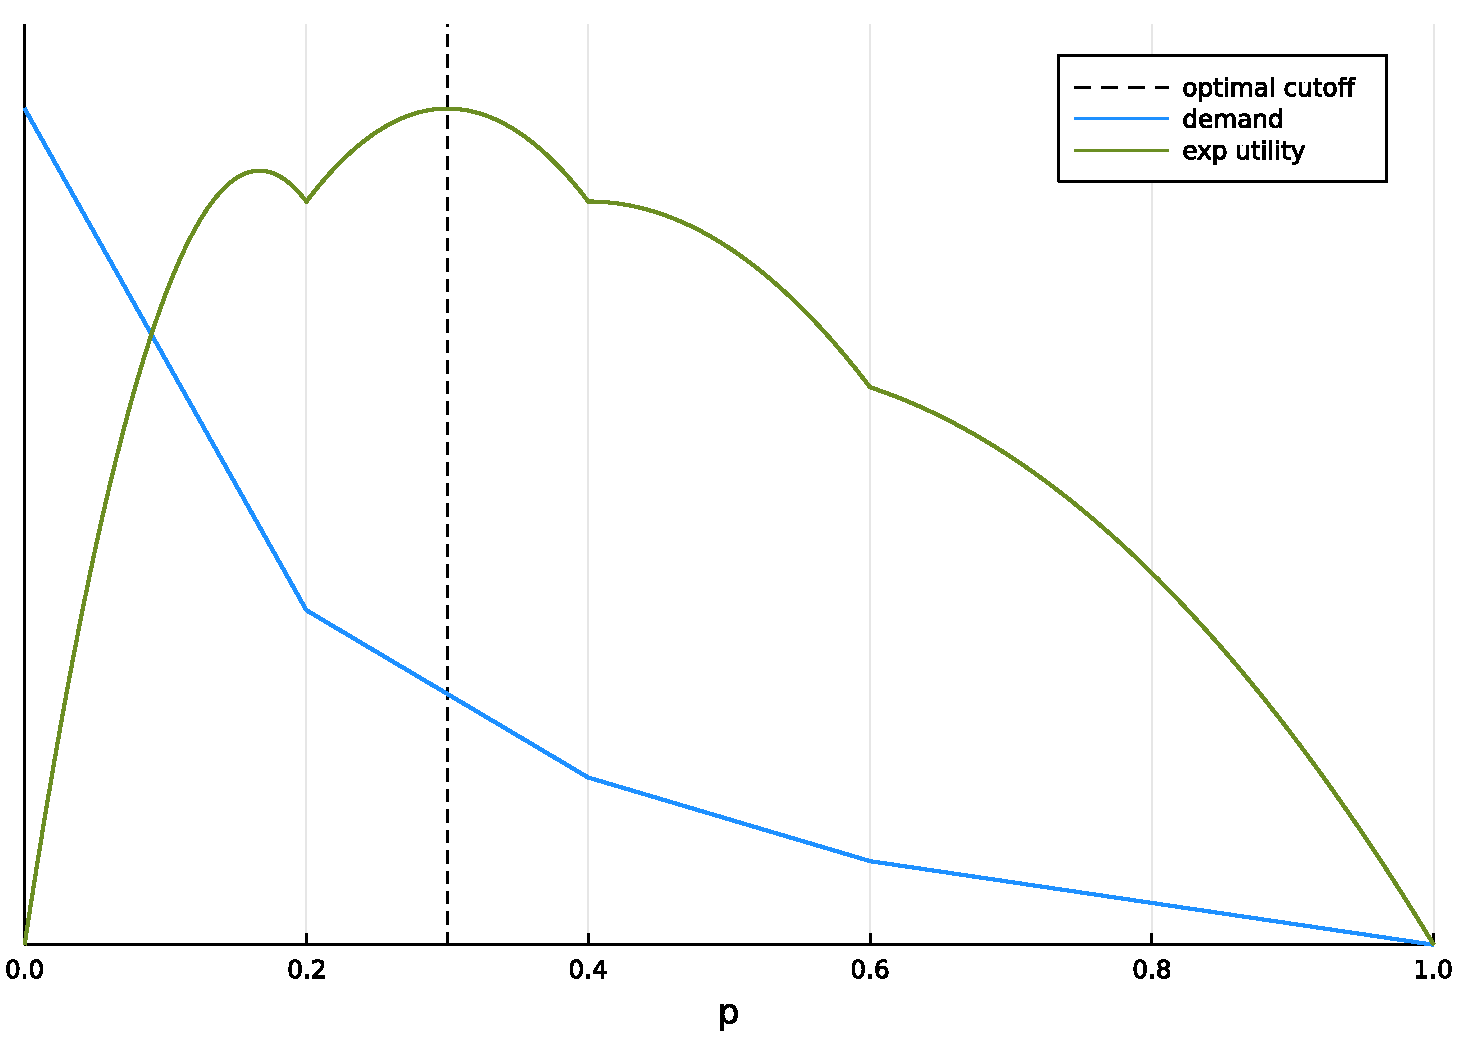
\includegraphics[width=\linewidth, ]{singlescoreplots/cloud-function-example.pdf}\end{center}
\captionsetup{singlelinecheck=off}
    \caption[.]{An example of the school utility function considered here. The plot shows the demand and utility at school 2 as a function of its cutoff when $\sigma_2 = 1$ and the market parameters are $\gamma = (1, 3, 2, 6)$ and $p = (0.2, p_2, 0.4, 0.6)$. The utility, shown in green and exponentiated for legibility, is piecewise concave, and thus to compute the school's best response, it suffices to maximize the utility within each piece, then compute the overall maximum. In this case, $\operatorname{BR}_2(p_{c'}) = 0.3$, as shown by the black dashed line. For comparison, the demand function appears in blue.}
\label{cloud-function-example}
\end{figure}



\subsection{Best-response dynamics can cycle}
Given an initial cutoff vector $p^{(0)}$, suppose that each admissions cycle, each school updates its cutoff to the value that maximizes its utility function under the assumption that the other schools' cutoffs remain the same. In the literature on externality games, such an iterative scheme is called the \emph{best-response dynamics}. 
\begin{equation} \label{bestresponsedynamics}
p_c^{(t+1)} \equiv \operatorname{BR}_c  (p_{c'}^{(t)}), \quad \forall c \in C
\end{equation}
Any fixed point of the best-response dynamics is a Nash equilibrium, and vice versa. The best-response dynamics are known to converge for many types of games, including so-called potential games in which each school's utility function can be interpreted as the gradient of a scalar-valued, convex potential function \parencite[][chap. 19]{algorithmicgametheory}. However, Memphis markets are not potential games, and the best-response dynamics can cycle. For example, in the market with $\gamma = (2, 4, 2)$ and $\sigma = (1, 1, 1)$, the cutoff vectors $p^{(0)} = \left(\frac{9}{32}, \frac{16}{32}, \frac{9}{32}\right)$ and $p^{(1)}= \left(\frac{12}{32}, \frac{16}{32}, \frac{12}{32}\right)$ are each other's best response. 

\subsection{Incentive-gradient dynamics reach a local equilibrium}
Given an initial cutoff vector $p^{(0)}$, suppose that each admissions cycle, each school updates its cutoff in the direction that locally improves its objective function according to a predetermined sequence of step sizes. I will call these the \emph{incentive-gradient dynamics}.
\begin{equation} \label{incentivegradientdynamics}
p_c^{(t+1)} \equiv p_{c}^{(t)} + \alpha_t u'_c(p_c; p_{c'}), \quad \forall c \in C
\end{equation}
Incentive-gradient dynamics are analogous to gradient ascent. Because each school's objective function is locally concave, when the sequence of step sizes $\alpha_t > 0$ satisfies the Robbins--Monro condition $\sum \alpha_t = \infty, \sum \alpha_t^2 < \infty$, these dynamics converge swiftly to a local equilibrium.

Computing the global Nash equilibrium of a Memphis market is a hard problem, and an effective algorithm combines a global search strategy based on best-response dynamics with a local search strategy based on analysis of each school's incentive gradient. 

% {A numerical example} section was here, but removed for brevity



\section{Inverse optimization of Memphis markets}
In this section, I consider the inverse optimization task, in which the demand of the market and the cutoff vector is provided and we attempt to compute the taste parameters $\gamma$ and $\sigma$. I provide an analytic solution for $\gamma$ that does not rely on an equilibrium assumption. Under the assumption that the market has attained a Nash equilibrium, I also provide an algorithmic solution for $\sigma$. Finally, I offer a proof-of-concept demonstration of the inverse optimization task using admissions data from 1073 American universities. 

\subsection{An analytic solution for the preferability parameters $\gamma$}
Given the demand $D$ and cutoff vector $p$, we aim to solve the following system for $\gamma$.
\begin{equation}
D_c = \sum_{d=c}^{|C|} 
\frac{\gamma_c}{ \sum_{i=1}^d \gamma_i} 
\left(p_{d+1} - p_{d}\right),
\quad \forall c \in C
 \label{solvemeforgamma}
 \end{equation}
Assume the schools are sorted in ascending order of cutoffs, and by homogeneity, let $\sum_{c \in C} \gamma_c \equiv 1$.

Consider the demand for $|C|$, the school with the highest index and therefore highest cutoff. Students who get into this school necessarily get into every school, so the outer sum of the system \eqref{solvemeforgamma} has only one term, and the equation becomes
\begin{align}D_{|C|} =
\frac{\gamma_{|C|}}{ \sum_{i=1}^{|C|} \gamma_i} 
\left(1 - p_{|C|}\right) \\
\implies \gamma_{|C|} = \frac{D_{|C|}}{1 - p_{|C|}}
\end{align}
Now suppose that we know $\gamma_{c+1}, \gamma_{c+2}, \dots, \gamma_{|C|}$. Then $\gamma_c$ can also be calculated from the observation that
\[\sum_{i=1}^d \gamma_i = 1 - \sum_{j=d+1}^{|C|} \gamma_j\]
where I take $\sum_{j=|C|+1}^{|C|} \gamma_j \equiv 0$.

Hence, the following recursive relation allows us to compute all the $\gamma_c$ values in reverse order, starting with $\gamma_{|C|}$ and moving down.
\begin{align}
\gamma_{|C|} &= \frac{D_{|C|}}{1 - p_{|C|}} \\[1em]
\gamma_c &= \frac{D_c}{~~\mathlarger{\sum_{d=c}^{|C|} \frac{p_{d+1} - p_d}{1 - \sum_{j=d+1}^{|C|} \gamma_j} ~~}}, \quad \forall c \in \bigl\{ |C|-1, |C|-2, \dots, 1\bigr\} \label{gammarecursion}
\end{align}
This calculation makes no equilibrium assumption. However, $p$ is a Walrasian equilibrium of any market for which school preferability parameters are given by this $\gamma$, $q_c \geq D_c$ for all schools, and $q_c = D_c$ for all schools with $p_c > 0$. 

\subsection{An algorithmic solution for the selectivity parameters $\sigma$}
Now, I impose an equilibrium assumption. The assumption of a Walrasian equilibrium leaves the inverse optimization problem underdetermined, because for a school with $p_c = 0$, its target demand $q_c$ can be arbitrarily higher than $D_c$ while still establishing an equilibrium. On the other hand, assuming that the market has attained a global Nash equilibrium, each school's selectivity parameter $\sigma_c$ can be computed algorithmically. 

Given the equilibrium cutoffs $p^*$ and preferability parameters $\gamma$, the Nash equilibrium is a stationary point of the best-response operator $\operatorname{BR}_c(p)$. The shape of each school's utility function depends only on the cutoffs and $\sigma_c$; thus, it suffices to solve the following $|C|$ univariate root research problems. 
\[\text{for each } c\text{, find } \sigma_c :\quad p^*_c = \operatorname{BR}_c  (p^*_{c'} ; \sigma_c) \]
If $\operatorname{BR}_c$ is monotonic and continuous in $\sigma_c$, then the root exists, is unique, and can be found using bisection. In a Memphis market, $\operatorname{BR}_c$ is strictly increasing in $\sigma_c$. That is, as $\sigma_c$ increases, so does the optimal cutoff $p^*_c$.  However, $\operatorname{BR}_c$ not continuous, and in certain cases, the discontinuity straddles the zero. When this happens, the bisection converges to the $\sigma_c$-value at the point of discontinuity. As the number of schools increases, the values of the best-response operator are typically quite small. 

The number of bisections $m$ required to achieve a given tolerance is independent of the number of schools in the market. Each bisection calls $\operatorname{BR}_c$ once, and each call is $\mathcal{O}(|C|^2)$, so the overall complexity of computing $\sigma_c$ for each school is $m \mathcal{O}( |C|^3)$.

\subsection{A demonstration using admissions data from American universities}
Here, I demonstrate the inverse optimization process using data from the Integrated Postsecondary Education Data System (IPEDS), a government database of information on American colleges and universities. The results and discussion below should be taken only as a proof of concept, for three reasons: First, this model makes the unrealistic assumption that all colleges have the same preference order, which is derived from students' standardized test scores. Second, I did not attempt to account for the fact that many students do not bother applying to schools for which they are are overqualified; as a result, the cutoffs are systematic underestimates. Finally, I excluded from consideration schools for which test statistics were not listed, reducing the dataset to 1073 school. Thus, whereas the inverse optimization procedure provided above estimates schools' \emph{preferability} and \emph{selectivity} when given perfect knowledge of their \emph{admissions standards}, in the present analysis, all three had to be estimated.

The IPEDS database contains information regarding students subscores on the SAT and ACT exams. For each test, the dataset shows the 25th and 75th percentile of scores among students admitted to each school. By comparing these percentiles to percentile tables released by the testing agencies, I derived one estimate of each school's cutoff value corresponding to each subscore. For example, at the certain college, the 75th-percentile ACT math score among admitted students is a 30 (out of 36). Relative to the population of ACT examinees, a student who earns a 30 is at the 90th percentile overall; hence, if this college looks only at ACT composite scores, it follows that the minimum score among its admits is at the 60th percentile among all test-takers. In the occasional case where this calculation yielded a negative value, I clamped the cutoff estimate to zero. Explicitly, letting $p_{\text{rel}}$ (here $0.75$) denote the percentile under consideration, and $p_{\text{abs}}$ (here $0.90$) denote the percentile score of a student with that score relative to the whole student population, the implied school cutoff is
\[p_{\text{impl}} = \max\left\{0, 1 - \frac{1 - p_{\text{abs}}}{1- p_{\text{rel}}}\right\}\]
To compute a composite estimate of each school's cutoff, I first averaged the cutoffs implied by the ACT and SAT data separately. Then, I took the average of these two weighted by the number of applicants who submitted each test score (which is also included in the IPEDS dataset) and treated this as the school's $p_c$.

To compute each school's demand, I divided the number of students enrolled at each school by the sum of the same. (In the tabular results and graphs, I report demand as a number of students instead of the proportion $D_c$ for legibility.) Thus, this model assumes that every student in the market can get into at least one college, and that the dataset includes all the college-like options that students in this market would consider. The first assumption is mild, because there are several colleges in the dataset whose estimated cutoff is zero. The second assumption is much more restrictive, as there are many colleges that do not report test scores, not to mention international schools, that are not represented in the data. Schools were excluded from analysis if fewer than three of the test-score indicators or class-size information was unavailable. 

For the data corresponding to each year from 2011 through 2019, I performed the preliminary calculations described above and computed the preferability vector $\gamma$ according to the inverse optimization procedure described above. I also estimated the $\sigma$-value corresponding to each school's objective function, but replaced the Nash equilibrium assumption with the arguably weaker assumption that each year, each school shifted its cutoff to its best response to the market conditions of the prior year. Thus, if the previous cutoffs were $p^{(t-1)}$, then $\sigma_c$ was computed according to the assumption that the value $p_c^{(t)}$ is $c$'s best response when the other schools' cutoffs are $p_{c'}^{(t-1)}$. This yielded an estimate of $\sigma$ for the years 2012 through 2019. Finally, I averaged the results over all years in order to obtain a composite estimate.\footnote{The code used to produce these results, along with additional data visualizations, is available on GitHub at \url{https://github.com/maxkapur/OneTest}.}

\subsubsection{Descriptive statistics}
The estimated preferability parameters $\gamma$ have an approximate log-normal distribution ($\text{mean} = 9.320 \times 10^{-4}$, $\text{sd} = 3.900 \times 10^{-3}$), as shown in Figure \ref{average-preferability-hist}. The selectivity parameters have $\gamma_c = 0$ for the nine schools whose average cutoff $p_c = 0$; the remaining $\sigma_c$-values also have an approximate log-normal distribution ($\text{mean} = 0.4819$, $\text{sd} = 4.1591$), shown in Figure \ref{average-selectivity-hist}.

Figure \ref{cutoff-demand-gamma-sigma-corr-heatmap} gives correlation coefficients among the parameters $p$, $D$, $\gamma$, and $\sigma$ in each year in the data set. While all the parameters are positively correlated, the strongest correlations are across years, suggesting the consistency of the derived measures. 


\begin{figure}
\begin{center}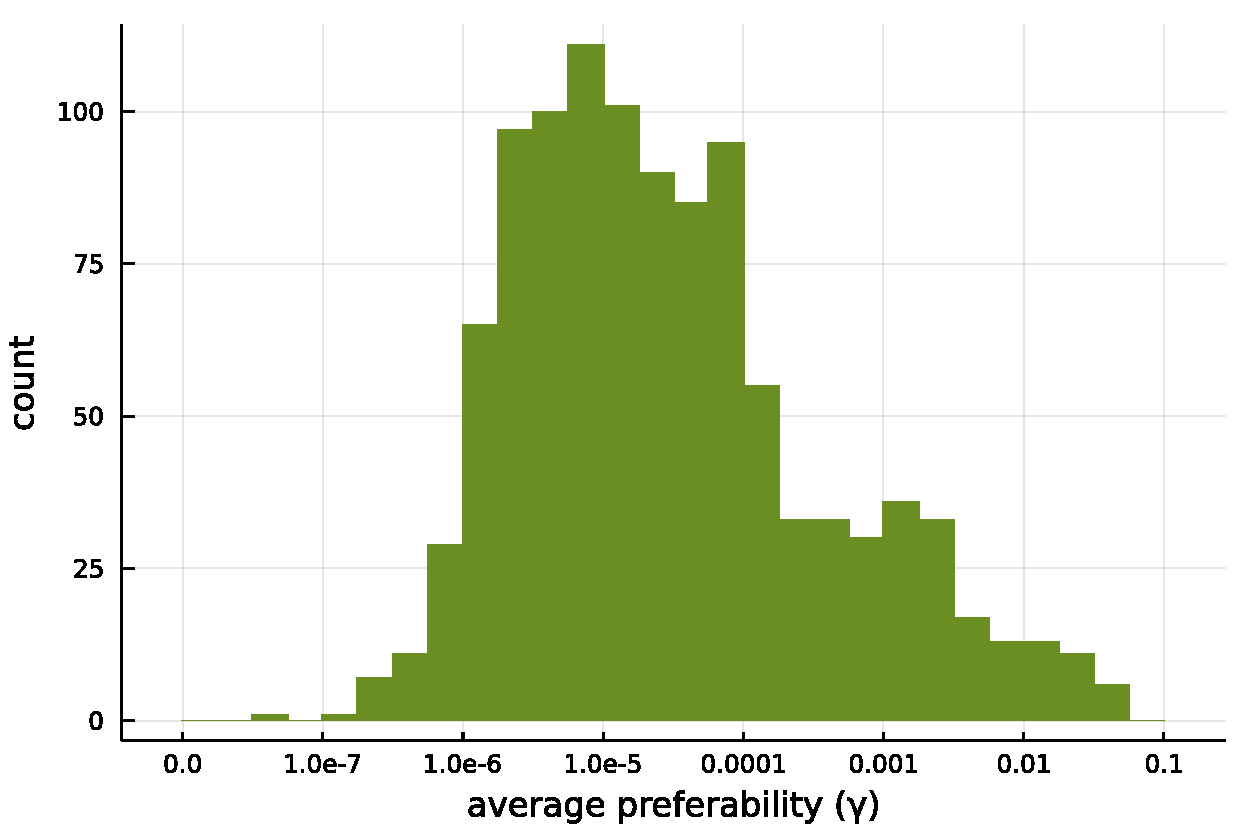
\includegraphics[width=\linewidth, ]{singlescoreplots/average-preferability-hist.pdf}\end{center}
\captionsetup{singlelinecheck=off}
    \caption[.]{Distribution of average preferability estimates $\gamma$ after applying the inverse optimization procedure to a public dataset describing 1073 American universities. The plot, shown on a log scale, suggests that the underlying parameters are normally distributed in the logarithm. }
\label{average-preferability-hist}
\end{figure}


\begin{figure}
\begin{center}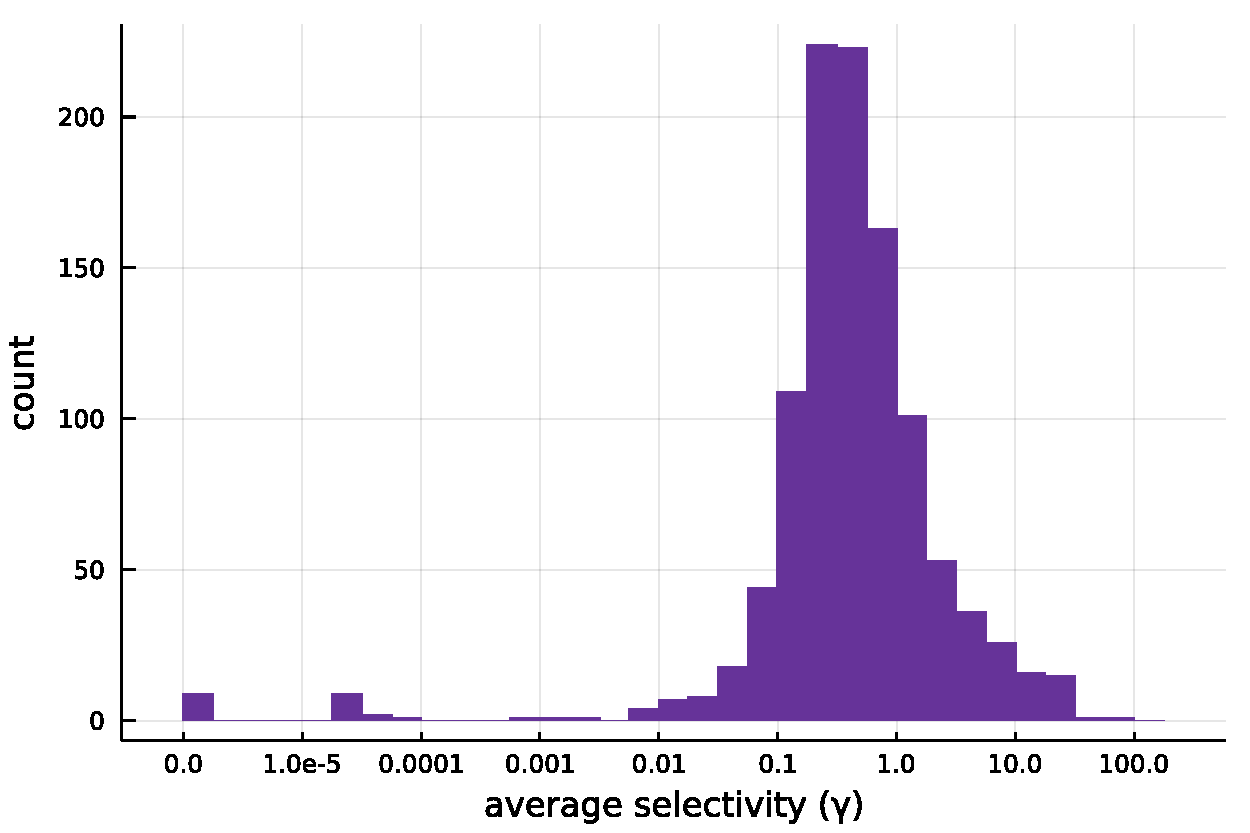
\includegraphics[width=\linewidth, ]{singlescoreplots/average-selectivity-hist.pdf}\end{center}
\captionsetup{singlelinecheck=off}
    \caption[.]{Distribution of average selectiveness estimates $\sigma$ after applying the inverse optimization procedure to a public dataset describing 1073 American universities. The plot, shown on a log scale, suggests that the underlying parameter distribution normal in the logarithm when schools for which $\sigma_c = 0$ are excluded.}
\label{average-selectivity-hist}
\end{figure}




\begin{figure}
\begin{center}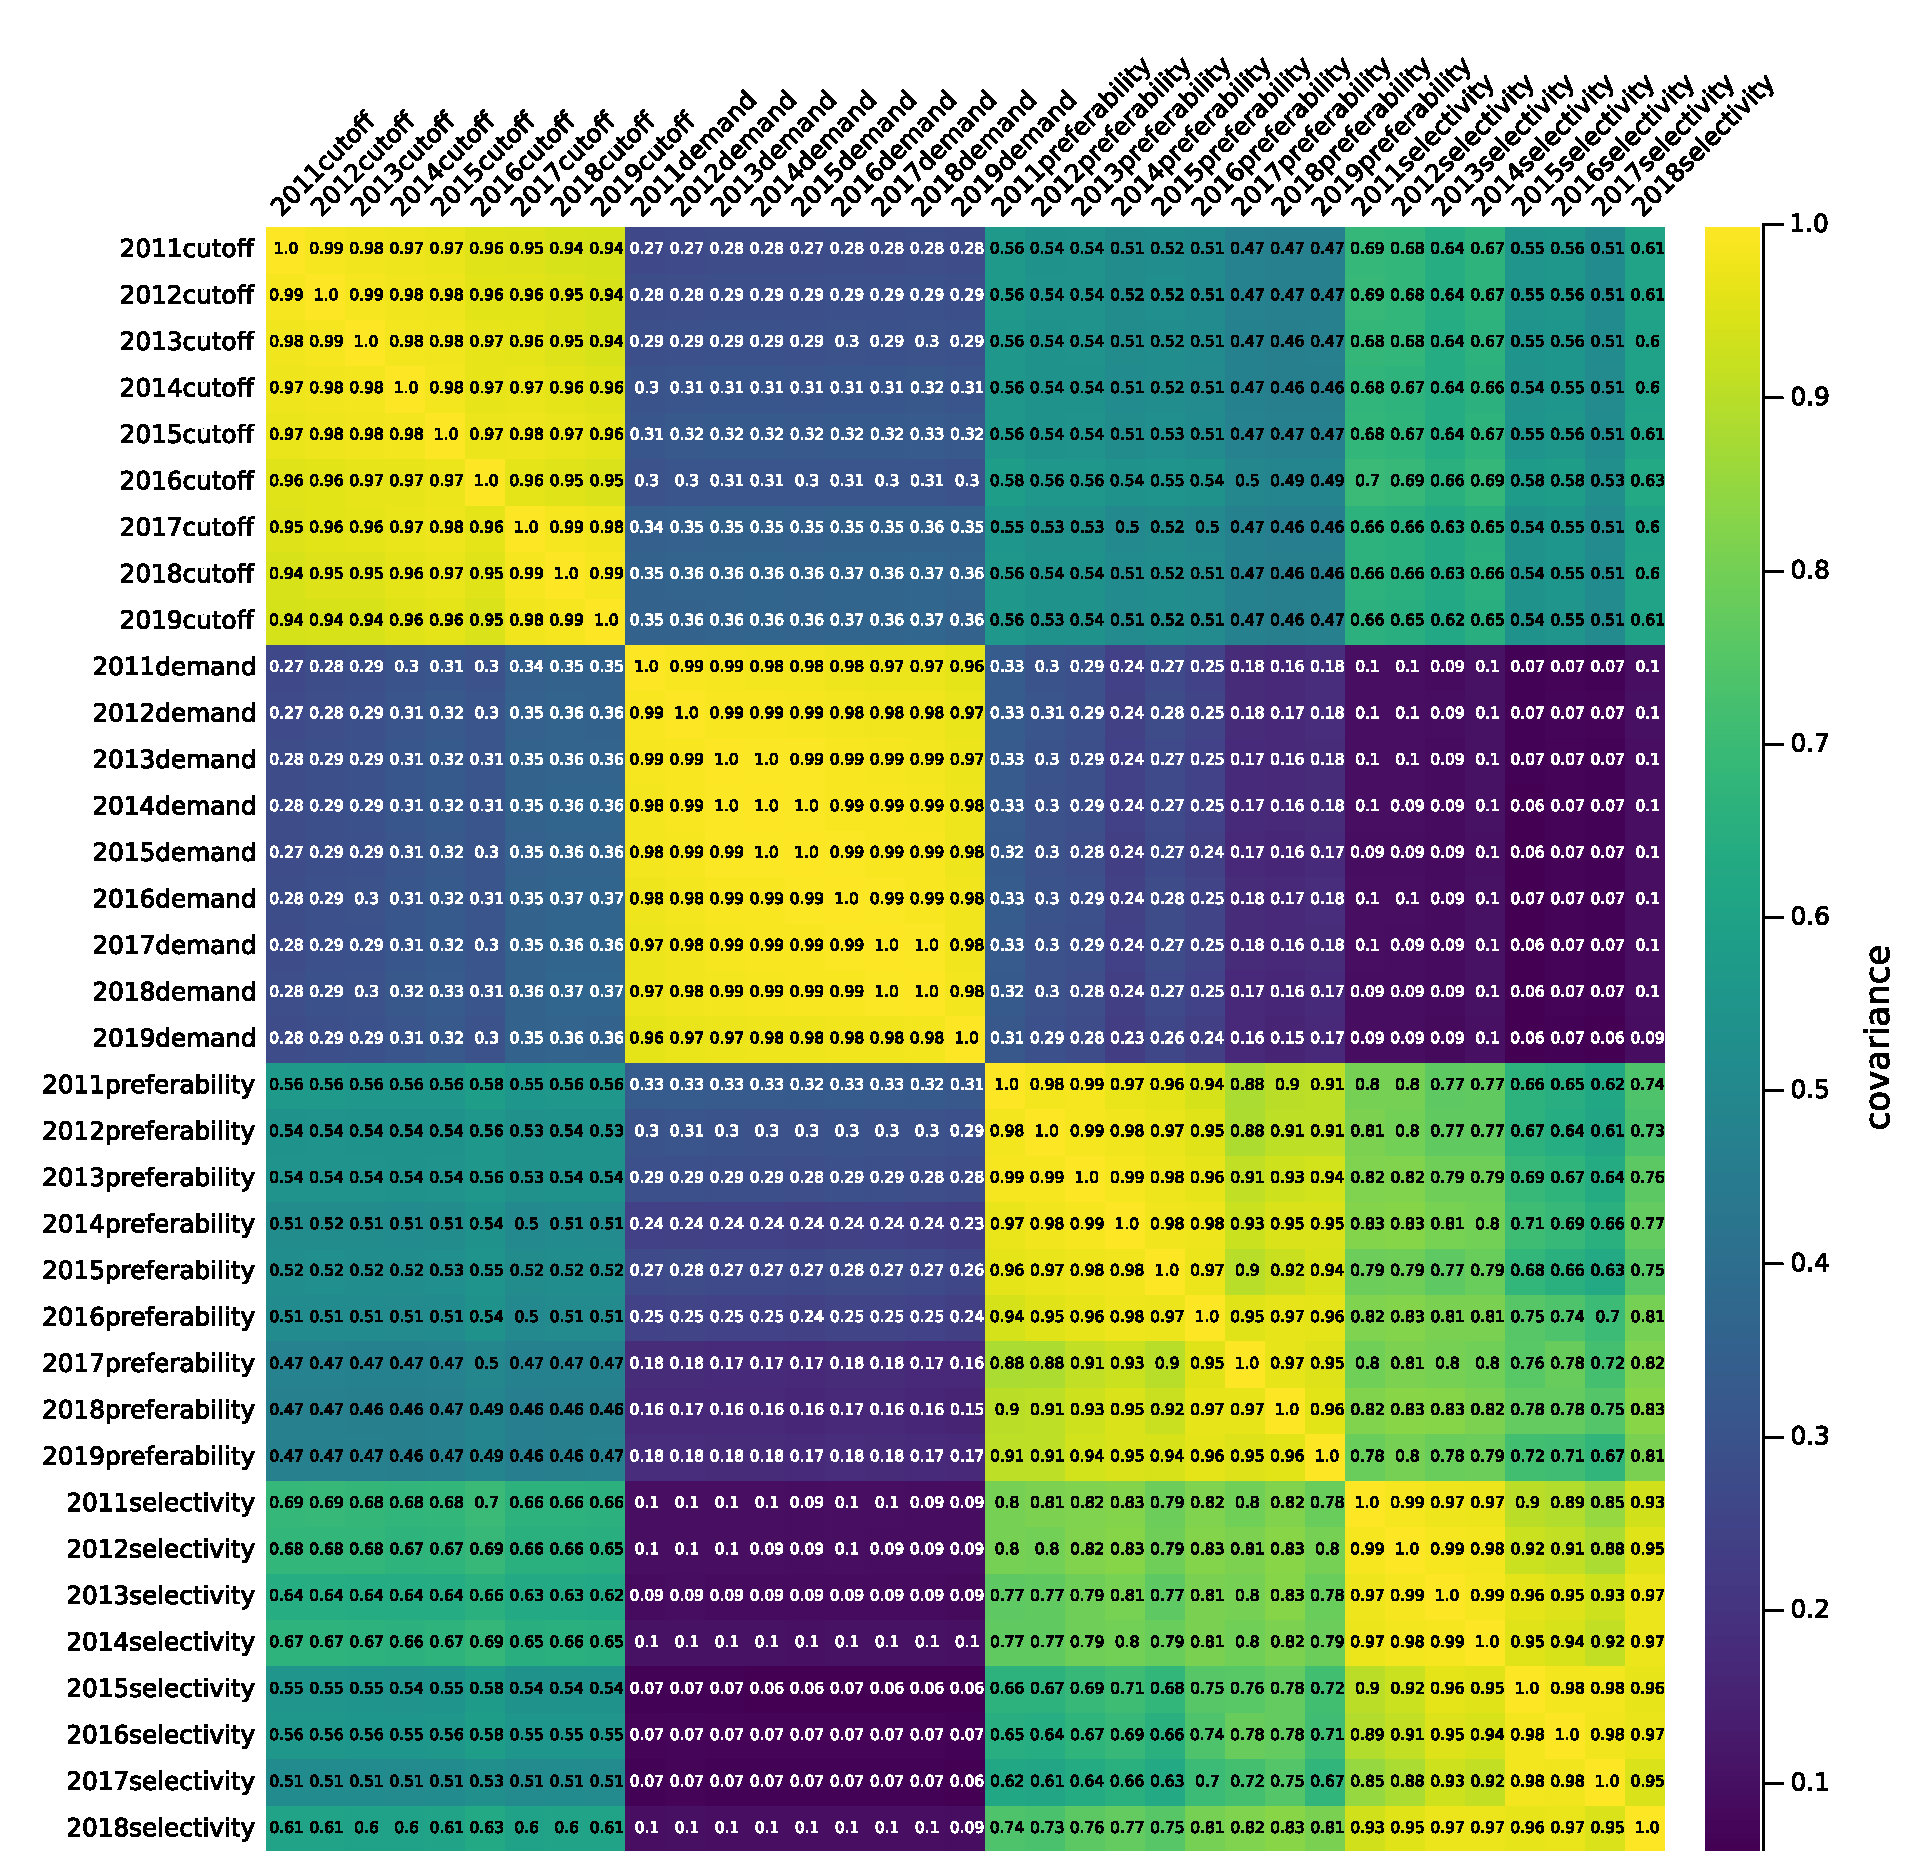
\includegraphics[width=\linewidth, ]{singlescoreplots/cutoff-demand-gamma-sigma-corr-heatmap.pdf}\end{center}
\captionsetup{singlelinecheck=off}
    \caption[.]{Correlation heatmap over the market parameters $p$, $D$, $\gamma$, and $\sigma$. While all four parameters are positively correlated, the strongest correlations are within each parameter and across data years.}
\label{cutoff-demand-gamma-sigma-corr-heatmap}
\end{figure}










\subsubsection{Ranking colleges}
The averaged results are shown in Figure \ref{US-cutoff-gamma} and Table \ref{tab:US-inverse-optimization}. The list of the schools with the highest preferability is a predictable list of prestigious universities. In a sense, this outcome is remarkable, because the input data contains no explicit indicators of ``prestige'' (such as data on endowment size and employment outcomes), nor any survey data akin to the questionnaires that some newspapers send to college executives to generate their rankings. The model also does not require observations of individual student choices, as used to estimate MNL parameters under traditional statistical paradigms. The preferability parameters simply emerge organically from the selectivity of each school, each school's total demand, and the assumptions about the distribution of student talent. For comparison, Table \ref{tab:US-inverse-optimization} provides other metrics that might be used to assess school preferability such as the demand, cutoff, yield (proportion of admitted students who choose to attend), and \emph{true yield.} The last is a contrived term for the proportion of \emph{qualified} students, regardless of whether they applied, who chose to attend the school; this can be computed from the cutoff and demand as $D_c / (1- p_c)$ . 

First, consider the top-ranked schools, whose figures are shown in Table \ref{tab:US-inverse-optimization}. Because this model considers not only selectivity but also entering class size as an indication of market power, compared to conventional college rankings, it grants an elevated position to public flagships like the University of Michigan at Ann Arbor, which draw large entering classes while maintaining fairly high admissions standards. Although tuition price has not figured into any stage of the analysis, this example shows that the computed preferability parameters incorporate a notion of \emph{value,} whereas traditional college rankings arrange schools as if their tuition prices are the same.

It is worth considering schools in other parts of the preferability distribution. While conventional wisdom posits small liberal-arts colleges and large public universities as incommensurable, administrators at both types of school share a common goal of recruiting an entering class that is both ``large'' relative to the physical size of the campus and ``highly qualified'' relative to competitor schools. $\gamma_c$ offers us a way to compare the effectiveness of two schools' marketing efforts even when their recruitment strategies diverge. For example, the University of Louisville (in Kentucky) and Whitman College (a liberal-arts college in eastern Washington) rank 156th and 157th, with average parameters $6.044 \times 10^{-4}$ and $6.001 \times 10^{-4}$, respectively. Louisville has a large class size and a middling cutoff, while Whitman has a small class size and a cutoff close to that the University of Illinois at Urbana-Champaign and Boston University. Looking only at conventional statistics, it is hard to predict the decision of a student choosing between the two schools, but comparing $\gamma$-values (which are, by definition, choice probability weights) reveals that in this case it is a nearly even coin flip. Indeed, the two schools' 2015 demand curves (shown in Figure \ref{three-demand-curves}) are all but identical. 

\subsubsection{Demand curve modeling}
The inverse optimization task makes no equilibrium assumption, and indeed invokes no notion of capacity or target class size. It simply reports the status of the market with respect to the current allocation of students. Thus, a possible application of this model is for an admissions director to use in modeling her school's demand curve. Figure \ref{three-demand-curves} shows the predicted demand curves for Louisville, Whitman, and Amherst College in the year 2015. This year, Amherst enrolled 471 students. Suppose that Amherst decides that a larger cohort of 600 students better suits its goals. By how much should it relax its admissions standards in order to achieve this class size? One way to answer this question is to assume that Amherst's true yield remains approximately fixed. Thus, Amherst should try to become $\frac{600}{471}$ more generous by updating its cutoff from the current value of $p_c = 0.9413$ to $1 - \frac{600}{471}(1 - 0.9413) = 0.9253$. A simple calculation shows that this yield-based estimate of the demand curve is equivalent to fitting a line to the observed demand $(p_c, D_c) = (0.9413, 471)$ and the implicit $x$-intercept $(1, 0)$. 

However, when using the yield-based model, the recommended cutoff associated with the higher target demand will be a slight underestimate, because Amherst's true yield also varies as a function of $p$. Under the proposed cutoff, students admitted with scores of (say) $0.935$ are admitted to Amherst but \emph{not} to competitor schools Notre Dame and Johns Hopkins, so Amherst will not have to compete as fiercely to recruit them as it does to recruit its current enrollees. The demand curve drawn by the Memphis model accounts for this change in the consideration set of marginal students, and thus it calls for a more modest reduction in Amherst's cutoff, to the value of $0.9314$.

Figure \ref{caltech-demand-curve} presents a detailed view of Amherst's demand curve in a Memphis market alongside the yield-based model. The Memphis curve has a slightly bowed shape, which confirms the intuitive argument for a gentler relaxation of admissions standards in order to achieve lower target enrollment. In fact, every school’s demand curve in this model is piecewise linear convex, meaning that the yield-based model will always underestimate the demand at cutoffs lower than the observed point.

This analysis has not accounted for the hypothesis that possibility that the appeal of a liberal-arts college like Amherst stems from its small class size, in which case looser admissions standards also reduce the school's preferability, necessitating a lower cutoff after all. Thus, in practical decisionmaking a model like that presented here is unlikely to be competitive with colleges' in-house models, which incorporate specific observations of students who applied to the school and chose to attend another. However, an advantage of the current model is that it produces an informative approximation of the demand curve without using students' personal data. Thus, a school like Amherst can use it to model the demand curves of its \emph{competitor} schools, enabling a more sophisticated recruitment strategy. 




%\subsubsection{What is a liberal-arts college?}





\begin{figure}
\begin{center}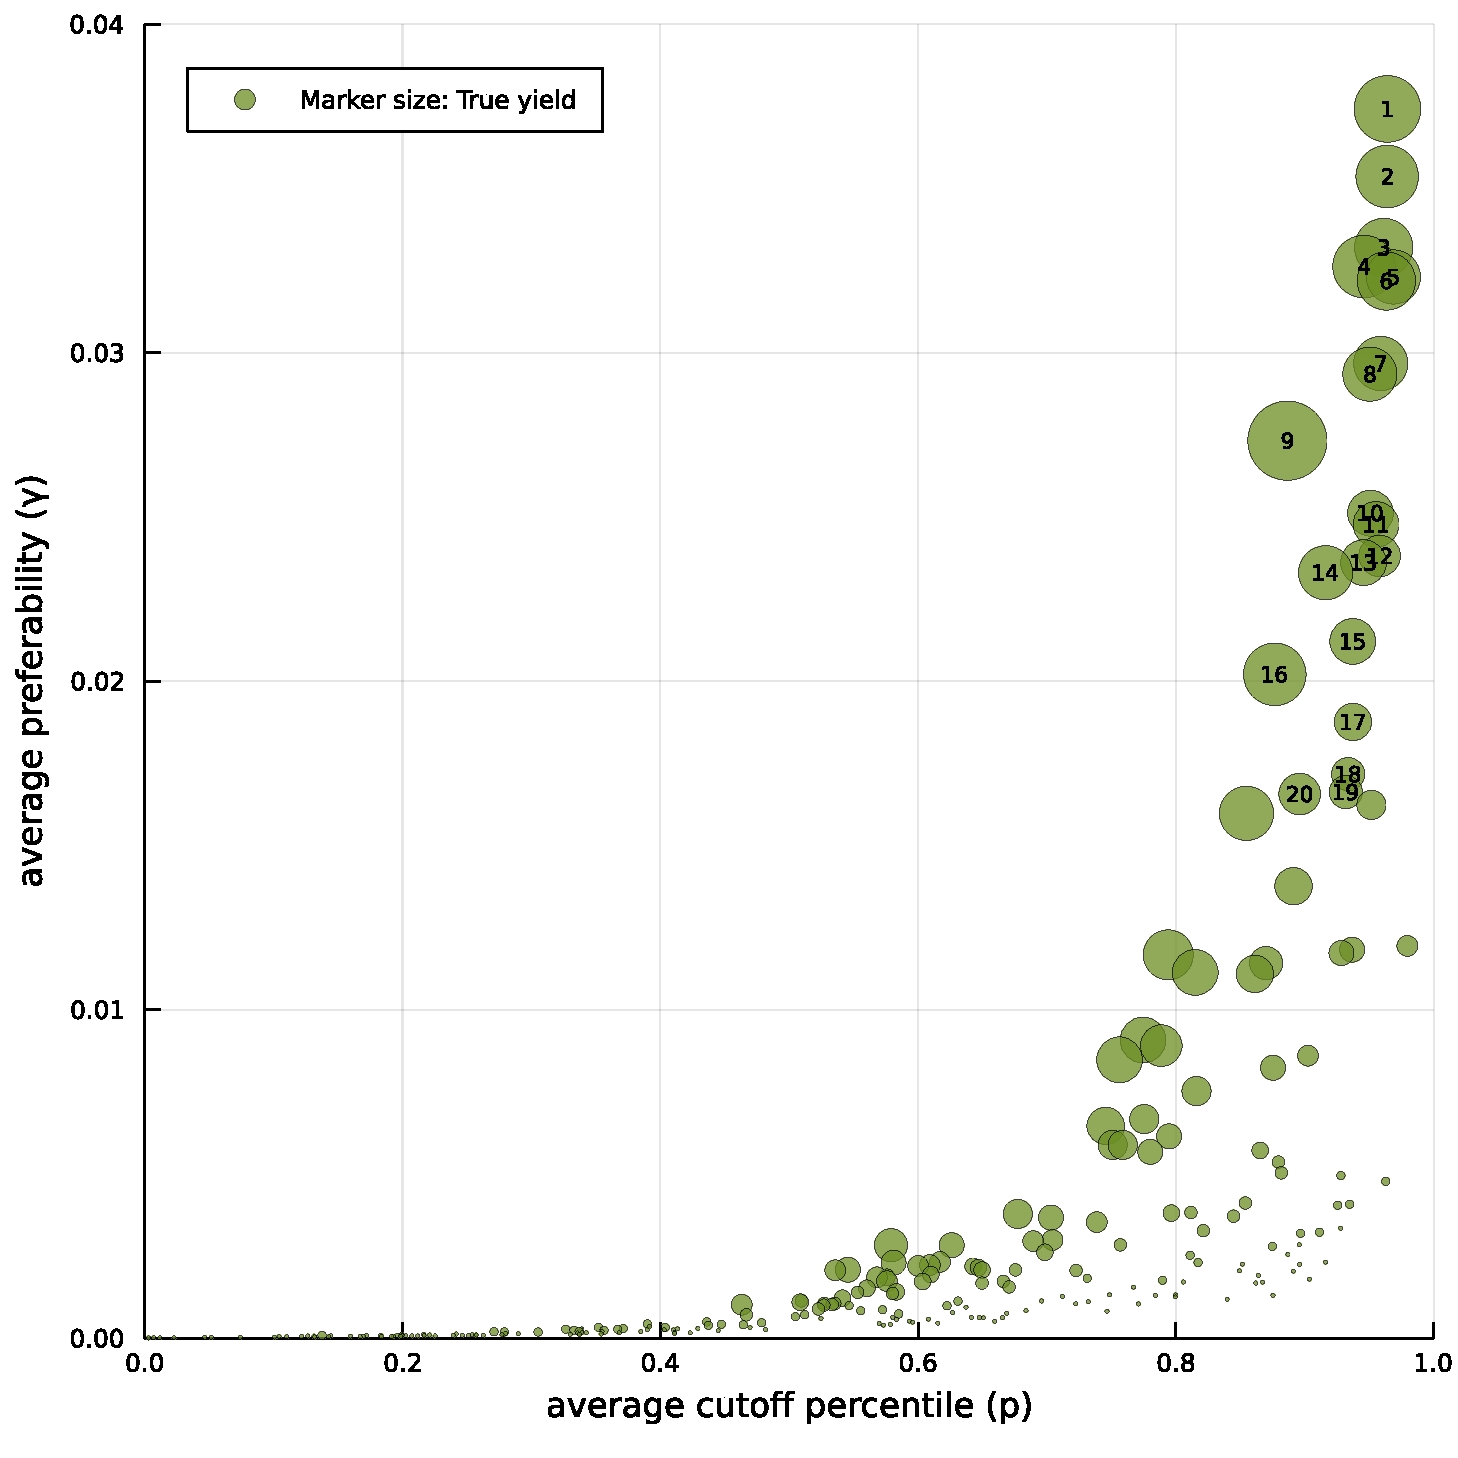
\includegraphics[width=\linewidth, ]{singlescoreplots/US-cutoff-gamma.pdf}\end{center}
\captionsetup{singlelinecheck=off}
    \caption[.]{Inverse optimization procedure applied to a dataset of 1073 American universities. School cutoffs were determined using a weighted average of cutoffs inferred from admitted students' SAT and ACT scores at the 25th and 75th percentiles. The marker size indicates the true yield, or percentage of qualified students who choose to attend each school. Details for the top twenty schools, as ranked by $\gamma_c$, appear in Table \ref{tab:US-inverse-optimization}.}
\label{US-cutoff-gamma}
\end{figure}




\begin{table}[]
\footnotesize \centering \begin{tabular}{r|lrrrrrr}
\textbf{\begin{tabular}[c]{@{}r@{}}Rank\\ ~ \end{tabular}} & \textbf{\begin{tabular}[c]{@{}r@{}}University\\~ \end{tabular}}                  & \textbf{\begin{tabular}[c]{@{}r@{}}Demand \\ ~\end{tabular}}& \textbf{\begin{tabular}[c]{@{}r@{}}Cutoff\\~ ($p_c$)\end{tabular}} & \textbf{\begin{tabular}[c]{@{}r@{}}Yield\\ ~ \end{tabular}} &  \textbf{\begin{tabular}[c]{@{}r@{}}True\\ yield\end{tabular}}  & \textbf{\begin{tabular}[c]{@{}r@{}}Pref.\\ ($\gamma_c$)\end{tabular}} & \textbf{\begin{tabular}[c]{@{}r@{}}Sel.\\ ($\sigma_c$)\end{tabular}} \\ \hline
1             & Harvard U                             & 1661            & 0.9641                                                         & 0.8074         & 0.0302              & 0.0374                                                                   & 29.71                                                                    \\
2             & U of Chicago                          & 1578            & 0.9639                                                         & 0.6146         & 0.0286              & 0.0354                                                                   & 29.29                                                                    \\
3             & Washington U in St. Louis              & 1698            & 0.9612                                                         & 0.3666         & 0.0274              & 0.0332                                                                   & 25.22                                                                    \\
4             & U of Pennsylvania                     & 2452            & 0.9459                                                         & 0.6532         & 0.0292              & 0.0326                                                                   & 19.15                                                                    \\
5             & Mass. Institute of Tech. & 1105            & 0.9687                                                         & 0.7265         & 0.0257              & 0.0323                                                                   & 39.05                                                                    \\
6             & Yale U                                & 1427            & 0.9633                                                         & 0.6784         & 0.0261              & 0.0322                                                                   & 28.48                                                                    \\
7             & Vanderbilt U                          & 1605            & 0.9589                                                         & 0.4375         & 0.0246              & 0.0297                                                                   & 24.59                                                                    \\
8             & Northwestern U                        & 2017            & 0.9505                                                         & 0.4738         & 0.0256              & 0.0293                                                                   & 19.95                                                                    \\
9             & U of Michigan--Ann Arbor               & 6475            & 0.8865                                                         & 0.4222         & 0.0362              & 0.0273                                                                   & 8.41                                                                     \\
10            & Stanford U                            & 1709            & 0.9509                                                         & 0.7837         & 0.0219              & 0.0251                                                                   & 20.46                                                                    \\
11            & Columbia U    & 1460            & 0.9553                                                         & 0.6066         & 0.0209              & 0.0248                                                                   & 22.88                                                                    \\
12            & Princeton U                           & 1318            & 0.9580                                                          & 0.6601         & 0.0198              & 0.0238                                                                   & 23.83                                                                    \\
13            & Duke U                                & 1734            & 0.9456                                                         & 0.4858         & 0.0210              & 0.0236                                                                   & 19.46                                                                    \\
14            & Cornell U                             & 3256            & 0.9161                                                         & 0.5397         & 0.0256              & 0.0233                                                                   & 12.50                                                                    \\
15            & U of Notre Dame                       & 2038            & 0.9372                                                         & 0.5444         & 0.0206              & 0.0212                                                                   & 15.85                                                                    \\
16            & U of California--Berkeley              & 5418            & 0.8767                                                         & 0.4230          & 0.0285              & 0.0202                                                                   & 7.77                                                                     \\
17            & Johns Hopkins U                       & 1406            & 0.9373                                                         & 0.3834         & 0.0168              & 0.0188                                                                   & 19.69                                                                    \\
18            & Brown U                               & 1600            & 0.9336                                                         & 0.5774         & 0.0164              & 0.0172                                                                   & 16.60                                                                    \\
19            & Carnegie Mellon U                     & 1524            & 0.9318                                                         & 0.3286         & 0.0158              & 0.0166                                                                   & 16.67                                                                    \\
20            & Northeastern U                        & 2878            & 0.8960                                                          & 0.2052         & 0.0197              & 0.0166                                                                   & 10.95                                                                   
\end{tabular}
\normalsize \caption{\label{tab:US-inverse-optimization}
The top twenty schools by average preferability $\gamma_c$, as determined by applying the inverse optimization process to a dataset of 1073 American universities over the years 2011 through 2019. Each school's demand is given as the average number of students in the entering class; to compute $D_c$, divide by the average total number of students, 1,266,305. The school's yield is the demand divided by the number of applicants reported by the admissions office, while the true yield, which represents the proportion of qualified students who chose to attend the school, was computed by comparing the size of the entering class to the estimated cutoff $p_c$.}
\end{table}





\begin{figure}
\begin{center}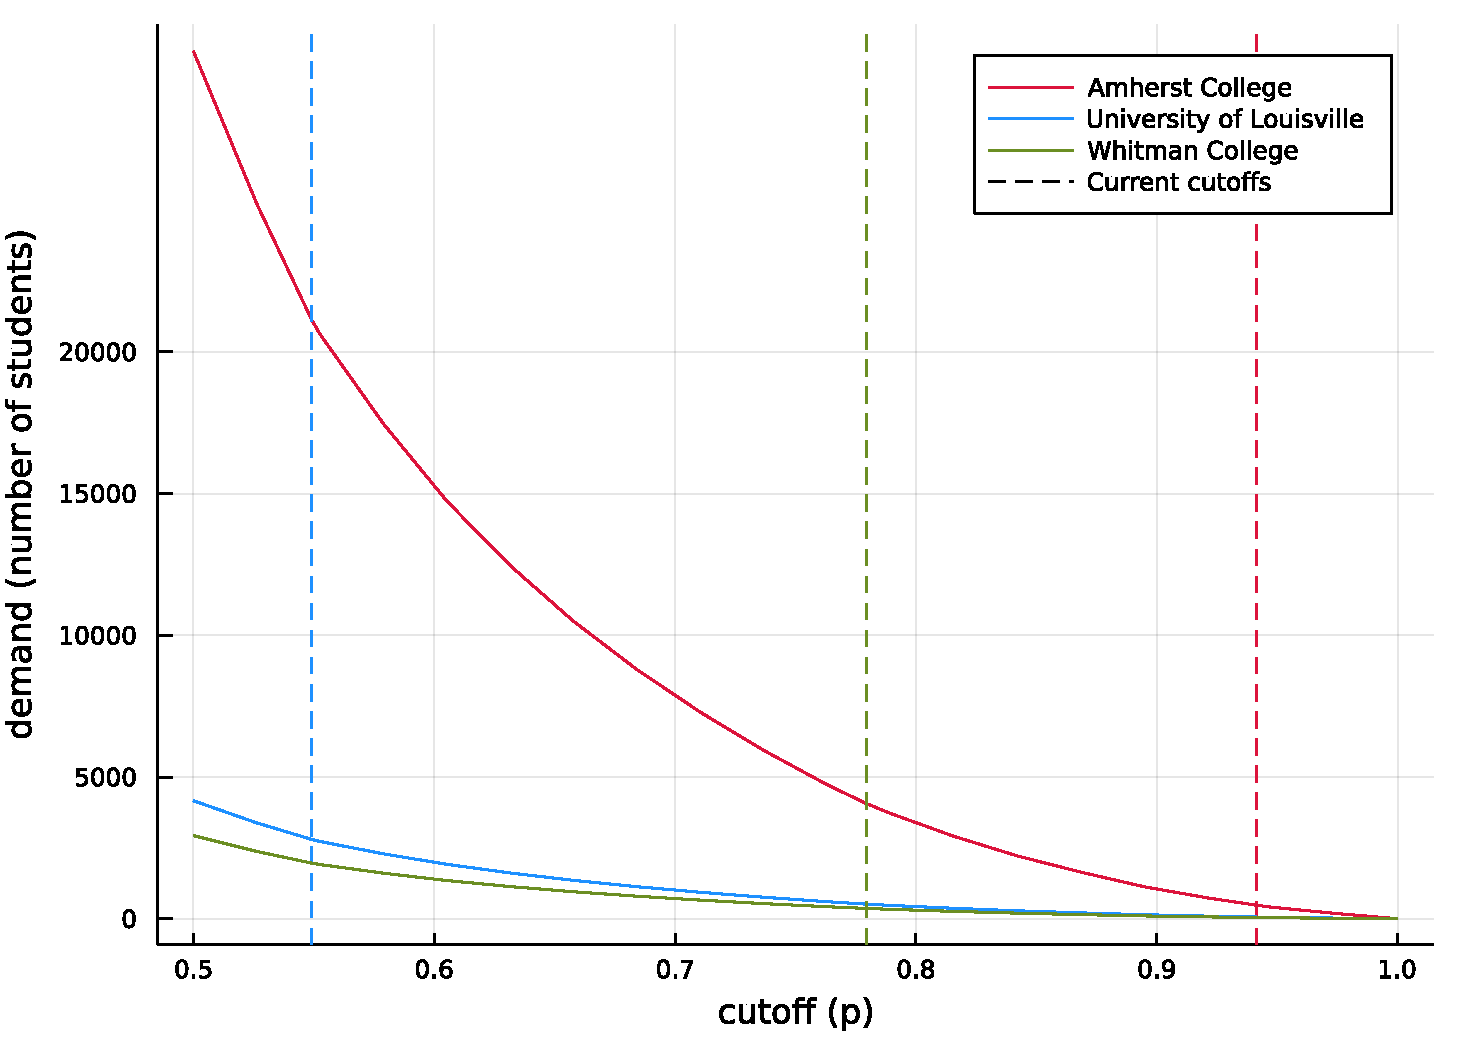
\includegraphics[width=\linewidth, ]{singlescoreplots/three-demand-curves.pdf}\end{center}
\captionsetup{singlelinecheck=off}
    \caption[.]{Three demand curves derived from 2015 data via the inverse optimization process. The University of Louisville and Whitman College have similar preferability parameters, and thus similar demand curves. However, each school has chosen a different selectivity threshold, reflecting its distinct admissions priorities. A detailed view of Amherst's demand curve appears in Figure \ref{caltech-demand-curve}.}
\label{three-demand-curves}
\end{figure}





\begin{figure}
\begin{center}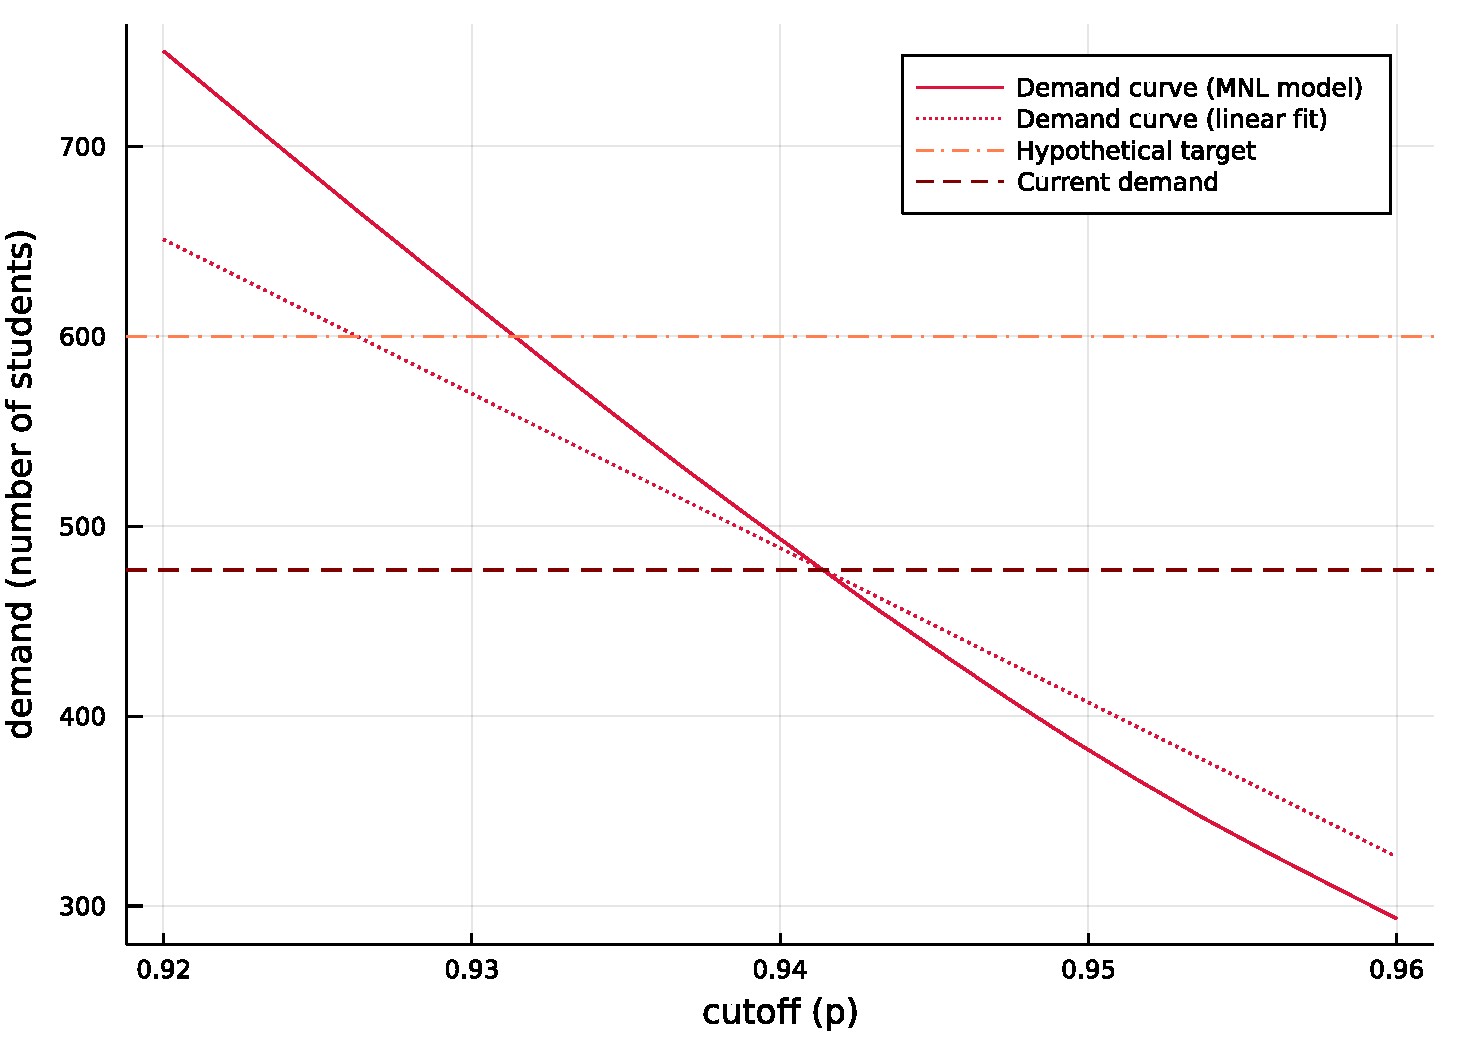
\includegraphics[width=\linewidth, ]{singlescoreplots/single-demand-curve.pdf}\end{center}
\captionsetup{singlelinecheck=off}
    \caption[.]{Detailed view of Amherst's demand curve near its 2015 cutoff. Assuming preferability and other schools' cutoffs remain fixed, if Amherst wishes to increase its class size to 700, it should update its cutoff to the value indicated by the intersection of the demand curve and the horizontal coral line. A linear model prescribes decreasing the cutoff to $p_c = 0.9253$, whereas the model provided here accounts for the fact that there is less competition for marginal students at the lower cutoff and prescribes a more conservative decrease to $0.9314$. }
\label{caltech-demand-curve}
\end{figure}










\subsection{The informational quality of $\gamma$ and the bias in yield}
The question of how to measure aggregate college preferability is not a simple one, and newspaper university rankings attract regular controversy for their imprecise methodology \parencite[][]{intlrankingsandconflicts}. Typical ranking metrics draw from a combination of survey data and performance measures of a university's quality such as its research output or data on alumni salaries. However, conducting accurate surveys is costly and difficult, and while performance measures may correlate with college preferability, they offer a normative indication of which colleges ``should'' be popular without accounting for the decisions students actually make---decisions that may depend less on hard facts than on intangible notions of fitness.

The traditional measure college administrators have used to quantify their school's preferability relative to others in the market has been the yield. As discussed above, colleges' \emph{true} yield (or another yield metric that corrects for applicant behavior) can be a useful tool in modeling the demand curve. However, as a measure of comparing the preferability of two different colleges, true yield systematically overrates lenient schools, which face less competition for students. For example, consider a market with only two schools, Lunar College ($p_1 = 0, D_1 =  \frac{100}{101}$) and Antarctic University ($p_2 = \frac{99}{100}, D_2 = \frac{1}{101}$). At both schools, the true yield is $D_c / (1 - p_c) = \frac{100}{101}$, a value that exaggerates the preferability of Lunar College by failing to account for the fact that the majority of its admits (and the vast majority of its enrollees) had no other option. The proportion of students who chose Lunar College \emph{over} Antarctic University is given by the former's preferability, $\gamma_1 = \frac{100/101 - 99/100}{1/100} = \frac{1}{101}$, while the preferability of Antartic University is $\gamma_2 = \frac{100}{101}$. This example, along with the demonstration above, suggests that insofar as $\gamma$ can be estimated accurately, it provides unbiased information about school preferability in a well-differentiated admissions market.

\section{Discussion}
This article has considered Memphis, a set of assumptions that yield an admissions market with many attractive numerical properties. Because each school shares the same ranking over the set of applicants, the number of possible consideration sets is small, and it is possible to efficiently compute demand curves for each school as a function of its admissions cutoff. The Walrasian equilibrium admits a closed-form expression. A Nash equilibrium that allows schools to express their preference for high-quality students relative to a large class size is also readily computable using best-response heuristics. Moreover, Memphis markets are conducive to parameter estimation. Though the Memphis model is too simplistic to match every contour of the American college admissions market, applying the inverse optimization procedure to publically available test score data yielded an intuitive ranking of top universities. The model also allows analyst to chart each school's demand curve without consulting granular data on individual students' enrollment decisions or imposing an equilibrium assumption.

Natural extensions of the computational model considered here include incorporating a more robust choice model, such as the nested or mixed MNL, and allowing for heterogeneous scoring across schools. Both of these modifications would allow for differentiation based on students' academic interests; for example, students interested in the performing arts systematically promote conservatories in their preference orders, and these schools in turn will score applicants according to different criteria. However, any departure from the homogeneous scoring assumption invites rapid multiplication in the number of possible consideration sets, in principle because it becomes impossible to construct a total ordering of the space of students.

The two notions of equilibrium treated in this paper were chosen for their computational tractability and theoretical interest. In general, the notion of a school's objective function is problematic, because it implies a cardinal and total ordering over the set of possible entering classes, when in reality even the weaker notion of a total ordering over applicants is difficult to defend \parencite[][]{collegeadmissionsisnotmarriage}.

Nonethless, in the real world, putatively decentralized admissions procedures may incorporate regulatory elements that push the market toward Walrasian equilibrium. For example, the college admissions procedure in South Korea can be viewed as a distributed approximation of the school-proposing deferred acceptance algorithm for stable assignment. In this model, the government places a firm limit, called an admissions quota, on the number of students who can attend each university. At the beginning of the admissions cycle, colleges are given the profiles of all the students interested in attending. Each college makes admissions offers over the course of several rounds, beginning with the highest-qualified students, and at each round a subset of the admitted students tentatively commits to attending one of the colleges that admitted them. This process continuous for three rounds, at which point most colleges have either filled their capacity, or bottomed out their pool of applicants. If students were allowed to apply to every college and there were infinite rounds, this would be equivalent to school-proposing DA. However, students are in fact allowed to apply to only six colleges, and colleges instate different evaluation criteria for students who rank the school with high priority. It would be interesting to quantify the welfare cost of these regulations relative to a true stable assignment procedure. A Memphis approximation of the Korean admissions market could be a useful analytic tool, because admissions decisions in Korea are based heavily on standardized test scores. 

This article has taken a microeconomic view of admissions markets that views the market as a closed system in which the set of schools and the distribution of student preferences are frozen. Thus, the results offered here are incommensurate with macroeconomic studies in the so-called Tiebout framework that model the sorting behavior of families who move in and out of admissions markets according to how much they value public education overall \parencite[][]{apuretheoryoflocalexpenditures, equilibriumandlocalredistribution}. Because this area of the literature includes comparisons across districts that use different assignment mechanisms, it would be worthwhile to examine the relationship between sorting behavior and choice mechanisms, whereas previous regression studies have treated sorting behavior as a dependent variable that must be controlled for \parencite[][]{doescompetitionamongpublicschools}.

\pagebreak
\section{References}
\printbibliography[heading=none]

\end{document}

